
%----------------------------------------------------------------------------------------
%	PACKAGES AND OTHER DOCUMENT CONFIGURATIONS
%----------------------------------------------------------------------------------------

\documentclass[twoside,11pt,a4paper,openright]{Thesis} % The default font size and one-sided printing (no margin offsets)[11pt, oneside]

\graphicspath{{Pictures/}} % Specifies the directory where pictures are stored


\usepackage[square, numbers, comma, sort&compress]{natbib} % Use the natbib reference package - read up on this to edit the reference style; if you want text (e.g. Smith et al., 2012) for the in-text references (instead of numbers), remove 'numbers'

\hypersetup{urlcolor=blue, colorlinks=true} % Colors hyperlinks in blue - change to black if annoying
\title{\ttitle} % Defines the thesis title - don't touch this

\begin{document}

\frontmatter % Use roman page numbering style (i, ii, iii, iv...) for the pre-content pages

\setstretch{1.3} % Line spacing of 1.3

% Define the page headers using the FancyHdr package and set up for one-sided printing
\fancyhead{} % Clears all page headers and footers
\rhead{\thepage} % Sets the right side header to show the page number
\lhead{} % Clears the left side page header

\pagestyle{fancy} % Finally, use the "fancy" page style to implement the FancyHdr headers

\newcommand{\HRule}{\rule{\linewidth}{0.5mm}} % New command to make the lines in the title page

% PDF meta-data
\hypersetup{pdftitle={\ttitle}}
\hypersetup{pdfsubject=\subjectname}
\hypersetup{pdfauthor=\authornames}
\hypersetup{pdfkeywords=\keywordnames}

%----------------------------------------------------------------------------------------
%	TITLE PAGE
%----------------------------------------------------------------------------------------

\begin{titlepage}
\begin{center}

%\textsc{\LARGE \univname}\\[0.5cm] % University name
\textsc{\LARGE Engineering Internship Report}\\[0.1cm]
{\Large 03/10/2014  $\sim$  09/09/2014}\\[0.5cm] % Thesis type

\HRule \\[0.4cm] % Horizontal line
{\textbf{\huge  \ttitle}}\\[0cm] % Thesis title
\HRule \\[2.5cm] % Horizontal line

\begin{figure}[htbp]
	\centering
		
\includegraphics[width=\textwidth,height=\textheight,keepaspectratio]{Figures/logo.png}
\end{figure}
\vspace{2.2cm}

\emph{\LARGE Author:}\\[0.2cm]
{\LARGE\authornames}\\[2.8cm]% Author name - remove the \href bracket to remove the link


%\emph{\Large Industrial Supervisor:} \\
%{\supname} \\% Supervisor name - remove the \href bracket to remove the link
%{\supnamex} \\% Supervisor name - remove the \href bracket to remove the link
%{\supnamexx}\\[0.5cm] % Supervisor name - remove the \href bracket to remove the link

%\emph{\Large Academic Supervisor:}\\
%{\examname} \\[2cm]% Author name - remove the \href bracket to remove the link

\large \textit{A report submitted in fulfilment of the requirements\\ for the degree of \degreename}\\[0.3cm] % University requirement text
\textit{at}\\[0.4cm]
{\Large \groupname}\\[2.5cm] % Research group name and department name

{\large \today}\\[4cm] % Date
%\includegraphics{Logo} % University/department logo - uncomment to place it

\vfill
\end{center}
\cleardoublepage
\end{titlepage}

%----------------------------------------------------------------------------------------
%	SUPERVISORS
%----------------------------------------------------------------------------------------
\setstretch{1.5} % Reset the line-spacing to 1.5 for body text (if it has changed)

\supervisors{\addtocontents{toc}{\vspace{1em}} % Add a gap in the Contents, for aesthetics
\vspace{1cm}

\emph{\Large Industrial Supervisors:}\\[0.5cm]
{\supname} \\% Supervisor name - remove the \href bracket to remove the link
Ingénieur Développement, \ \ Orange/IMT/OLPS/SMA/DM2E/CARE\\
Tel : 04.76.76.42.20\qquad E-mail : \href{mailto:matthieu.anne@orange.com}{matthieu.anne@orange.fr}\\[0.3cm]

\emph{\Large Academic Supervisor:}\\[0.5cm]
{\examname} \\
Directeur de EI-SE\\
Université Pierre et Marie Curie - LIP6\\
Tel : 01.44.27.96.35\qquad E-mail : \href{mailto:andrea.pinna@lip6.fr}{andrea.pinna@lip6.fr}
}

%----------------------------------------------------------------------------------------
%	ACKNOWLEDGEMENTS
%----------------------------------------------------------------------------------------

\cleardoublepage

\acknowledgements{\addtocontents{toc}{\vspace{1em}} % Add a gap in the Contents, for aesthetics
The internship opportunity I had with CARE group was a great chance for learning and professional development. It’s here at Orange Labs I strengthened my willing to future research careers. Therefore, I consider myself as a very lucky individual as I was provided with an opportunity to be a part of it. I am sincerely grateful for having a chance to meet so many wonderful people and professionals who led me through this six-month internship.

First and foremost, I would like to express my sincere gratitude to my supervisor M. Matthieu ANNE, for the continuous support of my internship, for his patience, motivation, and immense knowledge. His guidance helped me in all the time of research and writing of this report. I could not have imagined having a better superadvisor and mentor for my internship.

My sincere thanks also goes to M. Julien Roland, M. Marc Douet, who provided me their knowledge and experience and precious time, only with their help I can get better work enviroment.

Last but not the least, I would like to thank all the CARE team members. Thank you for the fabulous leisure time we had together!
}

%----------------------------------------------------------------------------------------
%	LIST OF CONTENTS/FIGURES/TABLES PAGES
%----------------------------------------------------------------------------------------
\pagebreak

\pagestyle{fancy} % The page style headers have been "empty" all this time, now use the "fancy" headers as defined before to bring them back

\lhead{\emph{Contents}} % Set the left side page header to "Contents"
\tableofcontents % Write out the Table of Contents

\addtocontents{toc}{\vspace{1em}} % Add a gap in the Contents, for aesthetics

\lhead{\emph{List of Figures}} % Set the left side page header to "List of Figures"
\listoffigures % Write out the List of Figures

%----------------------------------------------------------------------------------------
%	THESIS CONTENT - CHAPTERS
%----------------------------------------------------------------------------------------

\addtocontents{toc}{\vspace{1em}} % Add a gap in the Contents, for aesthetics

\mainmatter % Begin numeric (1,2,3...) page numbering

\setstretch{1.5} % Return the line spacing back to 1.5

\pagestyle{fancy} % Return the page headers back to the "fancy" style

% Include the chapters of the thesis as separate files from the Chapters folder
% Uncomment the lines as you write the chapters

% Chapter 1

\chapter{Introduction} % Main chapter title

\label{Chapter1} % For referencing the chapter elsewhere, use \ref{Chapter1}

\lhead{Chapter 1. \emph{Introduction}} % This is for the header on each page - perhaps a shortened title

%----------------------------------------------------------------------------------------

TR-069 (Technical Report 069) is a technical specification published by the \href{https://www.broadband-forum.org/}{Broadband Forum} and entitled CPE WAN Management Protocol (CWMP)\cite{tr069}. It defines an application layer protocol for remote management of end-user devices. As a bidirectional SOAP/HTTP-based protocol, it provides the communication between customer-premises equipment (CPE) and Auto Configuration Servers (ACS). It includes both a safe auto configuration and the control of other CPE management functions within an integrated framework. The protocol addresses the growing number of different Internet access devices such as modems, routers, gateways, as well as end-user devices which connect to the Internet, such as set-top boxes, and VoIP-phones. The TR-069 standard was developed for automatic configuration and management of these devices by Auto Configuration Servers (ACS). TR-069 was first published in May 2004, with amendments in 2006, 2007, 2010, July 2011 to version 1.3. and November 2013 to version 1.4 (am5)

On 23 October 2014, the new Smart Home product of Orange --Homelive-- has entered to the market. Homelive is a unique solution that can link to the connected objects in the home, allowing client to manage the appliances remotely. There are a range of connected devices: weather monitors, thermostats, light switches, sound and movement detectors, and smoke detectors. They are connected using the Z-Wave protocol. For Orange support team, managing and monitoring devices remotely is critical to reduce the maintenance fee.

The present report describes the work I have done during my six months’ internship at Orange Labs. In order to reduce the maintenance fee of sending support engineer to client homes, my mission was to evaluate the adaptation of TR-069 in the Homelive in order to remotely manage devices using an ACS. The following part of this chapter at first gives a basic conception of the context, then my internship objectives are presented. In the last section, the outline of the report will be listed.

%----------------------------------------------------------------------------------------

\section{Context}
\subsection{Smart Home}

Home automation \cite{homeautomation} is the residential extension of building automation. It is automation of the home, housework or household activities. Home automation may include centralized control of lighting, HVAC (heating, ventilation and air conditioning), appliances, security locks of gates and doors and other systems, to provide improved convenience, comfort, energy efficiency and security.

The popularity of home automation has been increasing greatly in recent years due to much higher affordability and simplicity through smartphone and tablet connectivity. The concept of the ``Internet of Things'' has tied in closely with the popularization of home automation. There are currently many communication protocol\footnote{Like Z-Wave, ZigBee, En-Ocean, etc.} for home automation.

A home automation system \cite{homeautomation1} integrates electrical devices in a house with each other. The techniques employed in home automation include those in building automation as well as the control of domestic activities, such as home entertainment systems, houseplant and yard watering, pet feeding, changing the ambiance "scenes" for different events (such as dinners or parties), lighting control system, and the use of domestic robots. Devices may be connected through a home network to allow control by a personal computer, and may allow remote access from the internet. Through the integration of information technologies with the home environment, systems and appliances can communicate in an integrated manner which results in convenience, energy efficiency, and safety benefits.

Orange contribution in standards aims at preparing an enhanced experience for the end-user, with a simplified approach in terms of in-home connectivity of the devices. It also targets an interoperable infrastructure, through a reference smart home architecture attracting various application providers, because the variety of relevant applications is a key element for the smart home market to take-off. This implies the availability of unified, open APIs proposed to the developers that do not want to deeply study each specific way to access the functionalities from all possible underlying technologies. Harmonization of data models is also a key standardization objective for Orange to propose smart home services in a seamless and progressive way to the end-user.
%------------------------------------------------------------------------------------------------------------------------------------------------------------
\subsection{Homelive Offer}

Homelive is a smart-home convenience system that puts their home at the customer’s fingertips when away. Using a single application accessed by a smartphone tablet or computer, Orange Homelive allows consumers to adjust settings and to control remotely all connected home appliances from any place in order to enhance home security, improve home comfort, and manage energy consumption in the home. Homelive includes support for a broad range of devices, and Orange is continuing to expand the types of services and devices supported. The home monitoring subscription service is available for 9.99 \euro per month, and sends alerts when devices such as motion detectors and smoke alarms are triggered to owners via SMS or email.

The Homelive pack is sold for 79 \euro ( \$99.00) with a special cash back offer of 78 \euro  offer is valid for all new Homelive customers. It includes a central unit and 3 devices — a smoke sensor, a door/window sensor and a motion sensor ( \fref{fig:1}). To enjoy the features of the Homelive solution, the user pays only 9.99 \euro  per month with a 12-month commitment. The subscription includes unlimited SMS alerts, continuity of service monitoring and alerts in case of internet failure (subject to Orange mobile coverage), dedicated technical support and storage of video and data for a month. The offer is not restricted to Orange customers. Homelive can be installed in any home in France with an active Internet connection.%(\fref{fig:2}).

\begin{figure}[htbp]
	\centering
		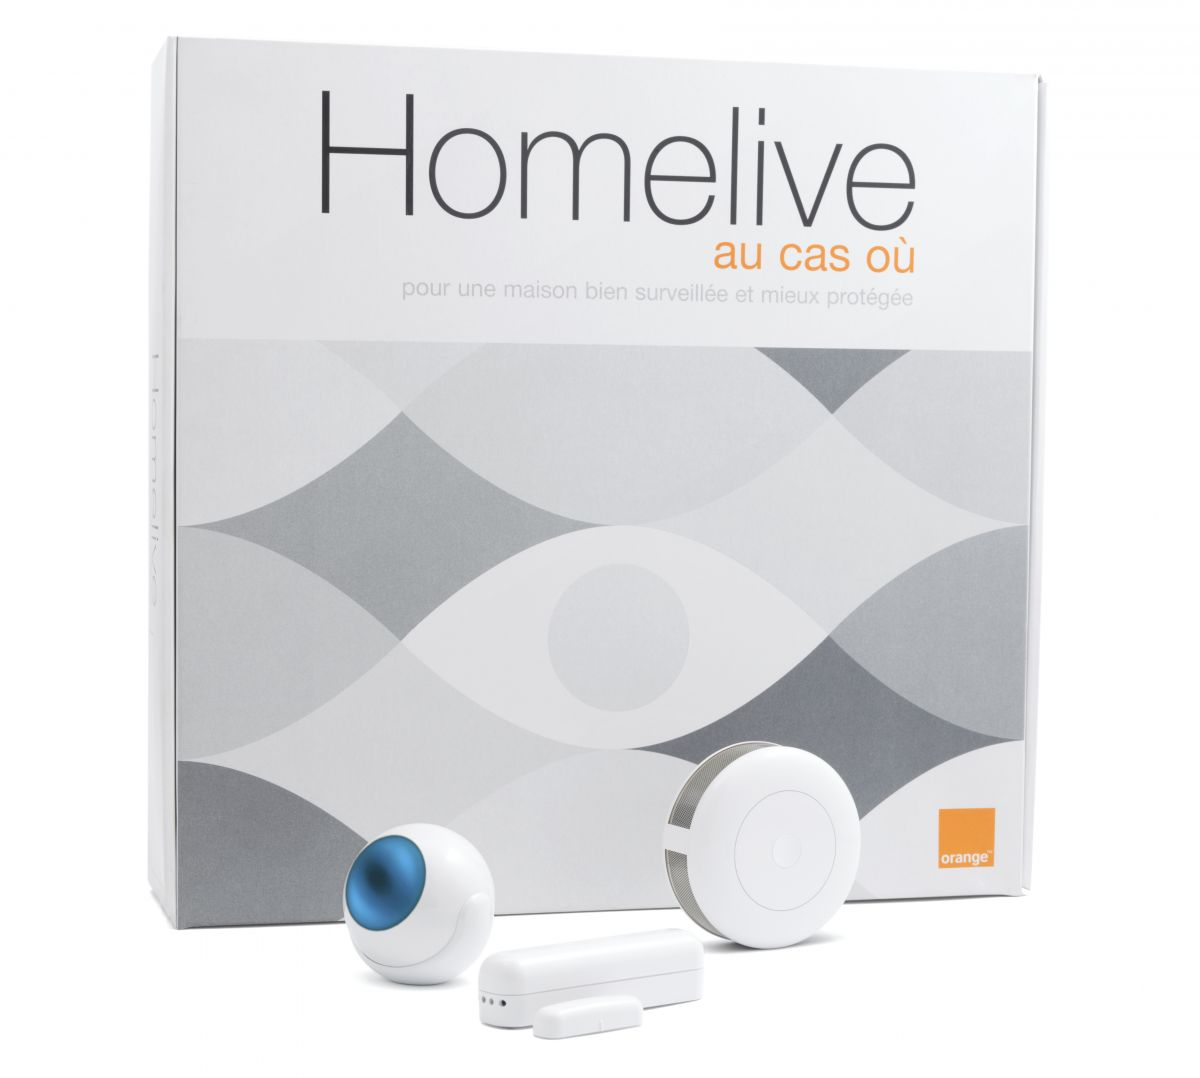
\includegraphics[width=10cm]{Figures/Pack_Accesoires_Homelive.jpg}
	\caption[Homelive ``Au Cas Où'']{Homelive ``Au Cas Où''}%{}
	\label{fig:1}
\end{figure}

\begin{figure}[htbp]
	\centering
		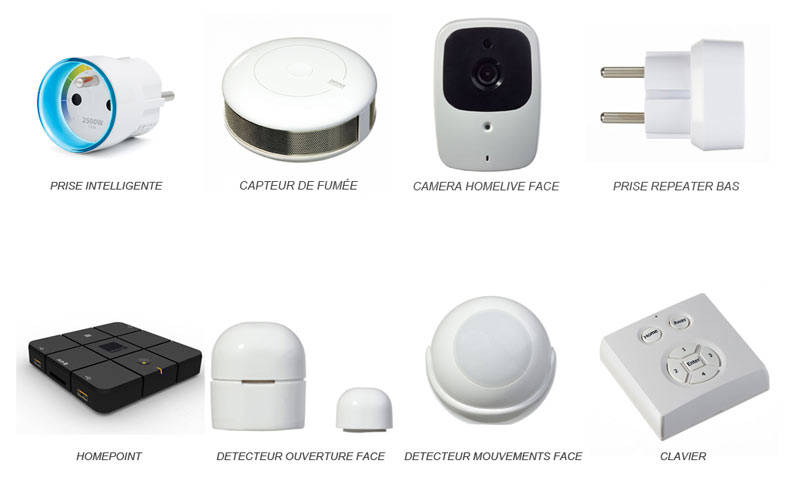
\includegraphics[width=10cm]{Figures/home-live_capteurs.jpg}
	\caption[Homelive Connected Object]{Homelive Connected Object}%{}
	\label{fig:2}
\end{figure}
%------------------------------------------------------------------------------
\subsection{Device Management}
A growing number of devices are connected in the user's home network and require device management. Service providers are faced with the new challenge of managing the increasing complexity of the home devices. Home Device Management addresses the technical device management and includes the following operations:
%------------------------------------------------------------------------------
\begin{itemize}
  \it
  \setstretch{1} % Reset the line-spacing to 1
  \item Setup and configuration of services (auto-provisioning),
  \item Managing connected devices (local or remote management): basic management, configuration management, software management, performance monitoring,
  \item Giving Service Providers more control (firmware upgrade),
	\item Cost reduction through remote management (avoid problem).
\end{itemize}
%------------------------------------------------------------------------------
Concerning the management of the connected devices, management could mainly be defined as follow:
\begin{itemize}
  \it
  \setstretch{1} % Reset the line-spacing to 1
  \item \textbf{Basic Management :} Enable reboot, baseline reset, logging and basic test features such as ping, traceroute, nslookup and self-test action.
  \item \textbf{Configuration Management :} Includes Data Model access and setting, i.e. parameter setting and object creation.
  \item \textbf{Software Management :} Enable Deployment Unit, i.e., installation/uninstallation/update of software package; Execution Unit, i.e., active unit, start and stop.
	\item \textbf{Performance Monitoring :} Include time base mechanism to retrieve information on the device behavior, i.e., raw, threshold or aggregated.
\end{itemize}
%------------------------------------------------------------------------------
Software vendors proposes several solutions to achieve these goals based on proprietary or standardized protocols. There are several standardization initiatives but the Broadband Forum is the more interesting proposal to address remote Home Device Management needs from the operator point of view.



The core protocol CWMP (CPE Wan Management Protocol, also known as TR-069) is specified in the Broadband Forum. The data models are produced by the Broadband Forum based on other organization inputs. Standard organization or forum like HGI\footnote{Home Gateway Initiative, smart home gateway provider.} or ETSI TISPAN\footnote{Telecoms \& Internet converged Services \& Protocols for Advanced Network.} proposes implementation profiles requiring certain parameters as mandatory.

Nevertheless, TR-069 is not well adopted by manufacturers, especially consumer electronic vendors. To achieve local Home Device Management the UPnP Forum has created a Working Committee dedicated to Device Management namely: \textbf{UPnP Device Management}. Orange is currently co-chairing it with Samsung. This working committee is defining a local management protocol which is able to cover the remote management scope, i.e., from a local/inner point of view, and to manipulate Data Model definitions coming from other forum such as Broadband Forum or OMA\footnote{Open Mobile Alliance who defines mobile phone specifications \& standards, enabling advancements in mobile across the globe.}.
%------------------------------------
\section{Objective of Internship}

Device management is a key asset for Orange used to upgrade the Livebox or Homelive firmware for new services deployment; it also used for VoIP activation and next generation liveradio \& IPTV set-top box. Orange is operating a TR69 platform named Karma. Under the situation that Homelive is growing in the market, device management based on TR-069 is become critical for Orange.

The principal objective of this internship is divided into two parts:
\begin{enumerate}
\it
\item Deploy the TR-069 client onto the Homelive Box of Orange and implementer the RPC methods.
\item Integrate the new data model Z-Wave in the TR-069 Client, and evolve it work under the HardWare//Firmware of Homelive Box.
\end{enumerate}
%----------------------------------------------------------------------------------------

\section{Outline}
In the first part( \autoref{Chapter2}) the enterprise Orange, and also the Orange Labs and the team CARE where I accomplish my internship will be introduced.

\autoref{Chapter3} will cover the several most important technical backgrounds. It first explains the \textit{CPE WAN Management Protocol (CWMP)} which defines several data models. Then is the Luup and MMS management platform which are provided by the main partner (Mios\footnote{MiOS, LTD. is a global software and hardware company represented in over 60 countries, and focused on developing and distributing advanced control and monitoring solutions for the home and small enterprise markets.}) of Orange on the Smart Home project. Also the \textit{NAT traversal} will be presented after Mios, it is a computer networking methodology with the goal to establish and maintain Internet protocol connections across gateways that implement \textit{Network Address Translation (NAT)}. At last, the Homelive box will be analyzed, including the hardware analyze, operating system OpenWRT and Cross-Compiling between working machine and the embedded system OpenWRT.

The following chapter( \autoref{Chapter4}) focuses on global architecture of Homelive Management Platform. The procedure of the communication between \textit{Auto Configuration Server (ACS)} and \textit{Customer-Premises Equipment (CPE)}will be described. Then, it goes over the position of my work in the whole project of the team.

\autoref{Chapter5} explains my work on the first objective of this internship---TR-069 Client. Firstly, due to the highly modularization, the architecture of the program TR-069 client will be introduced. Then is the problems I meet during the implementation of TR-069 Client and the solutions I proposed. The result of completion of the RPC methods will be listed at last.

The final \autoref{Chapter6} will present the second objective which is to integrate the data model Z-Wave in order to build the home network of connected objects and allow them to communicate with each other. The protocol and data model Z-Wave will be presented at first. Then is the procedure of synchronization of Z-Wave data model in Homelive firmware, TR-069 client and Automatic Configuration Server.

% Chapter 2

\chapter{Company Presentation} % Main chapter title

\label{Chapter2} % For referencing the chapter elsewhere, use \ref{Chapter2}

\lhead{Chapter 2. \emph{Company Presentation}} % This is for the header on each page - perhaps a shortened title


%----------------------------------------------------------------------------------------

\section{Presentation of Orange}
Orange, formerly France Telecom\cite{benilde2010portrait}, is a world-renowned French company specialized in the telecommunications sector. Orange has a rather eventful history due to multiple redemptions, but when France Telecom bought Orange PLC in August 2000, the group goes global. Orange has became the single brand of the group for the Internet, television and telephony (replacing Wanadoo, Itineris, Ola, Mobicarte ...). In 2006, Orange Business Services (OBS) appears to offer products and services to businesses and governments worldwide. At July 2013 that the France Telecom Group --- Orange takes the official name of \textbf{Orange}\cite{bertolus2003qui}.

\subsection{An International Operator}
Orange is the number three mobile operator and the number 1 ADSL television in Europe. The group is now present in 32 countries worldwide and strives to continue to deploy its foreign products and services . The operator carries much attention to the development of mobile services in Africa\cite{jaffre2005afrique} and the Middle East where it totals 88 million customers at 31 December 2013 (approximately 37\% of its customers). Some services Such "Orange Money" are deploying well abroad (8.9 million customers in Africa). Finally, since the arrival of 4G, Orange also invested in the coverage of European countries where customers are numerous (2 million customers in Poland and the UK in January 2014). Accordingly, Orange has 236 million customers worldwide (32 countries in 2014) while confused Service (76\% in mobile client) and employs 165000 people. The band has annual major case (about 41 billion euros in 2013).

%----------------------------------------------------------------------------------------

\section{Presentation of Orange Labs}
Innovation is a major growth lever for the Orange group. Research and development centers, also known as \textit{Orange Labs} form the group's innovation base. Today, 3,500 experts working within 18 Orange locations in 10 countries. In 2013, Orange continued its efforts in research and innovation by allocating 1.9\% of its turnover (780 million euros). Orange holds about 7,500 patents and apply 250 every year. Within the whole group, Orange employs 3700 people in research and development, and 200 PhD students and postdocs per year . The missions of research and development centers are:

\begin{itemize}
	\item The development of new quality products and services for the group,
	\item The release of new sources of growth with strong potential,
	\item The anticipation of technical and technological developments,
 	\item	The imagination of the solutions of the future with anticipation of long-term issues.
\end{itemize}

Orange is also widely involved in the many technical activities such as in standardization groups (eg 3GPP, IEEE or HGI) to be a major player in worldwide innovation.

%----------------------------------------------------------------------------------------
\section{Structure}
The company Orange is structured around various entities each with a specific role and specific occupations. Thus, the group consists of management entities, human resources management, communication, design, etc ... The entity Innovation, Marketing and Technologies (IMT) is responsible for giving a body to the operator in Internet era. Thus, IMT aims to digitize the operator in his close customer behavior, renewal of the various infrastructures and open the operation base station on the outside, based on innovation. This entity thus relies on innovation to differentiate themselves from the competition on marketing, to provide simple and reliable services and technologies and enrich its infrastructure.

IMT within various specialized research centers (Orange Labs Research), network (Orange Labs Networks), services (Orange Labs Products and Services), marketing (Technocentre), etc ... are responsible for delivering products and services focused on clients and their uses.

Composed of more than 3,000 people, Orange Labs Products and Services (OLPS) has overall technical responsibility for the products and services offered by Orange, the maintenance of implemented solutions in the world. Thus OLPS decomposes services that are more specific, such as SMA (SMart Access) which specializes in the domestic environment, SOFT which is specialized in the development of software components or UCE (Users and Customer Experience), which specializes in customer relationship. Each of these new services to decompose into smaller entities.

The chart below briefly presents how is structured Orange. There is more detailed for entities specialized in the design of new products and services, especially in the domestic field. The last level is the team working on the offer Smart Home Orange.

\begin{figure}[htbp]
	\centering
		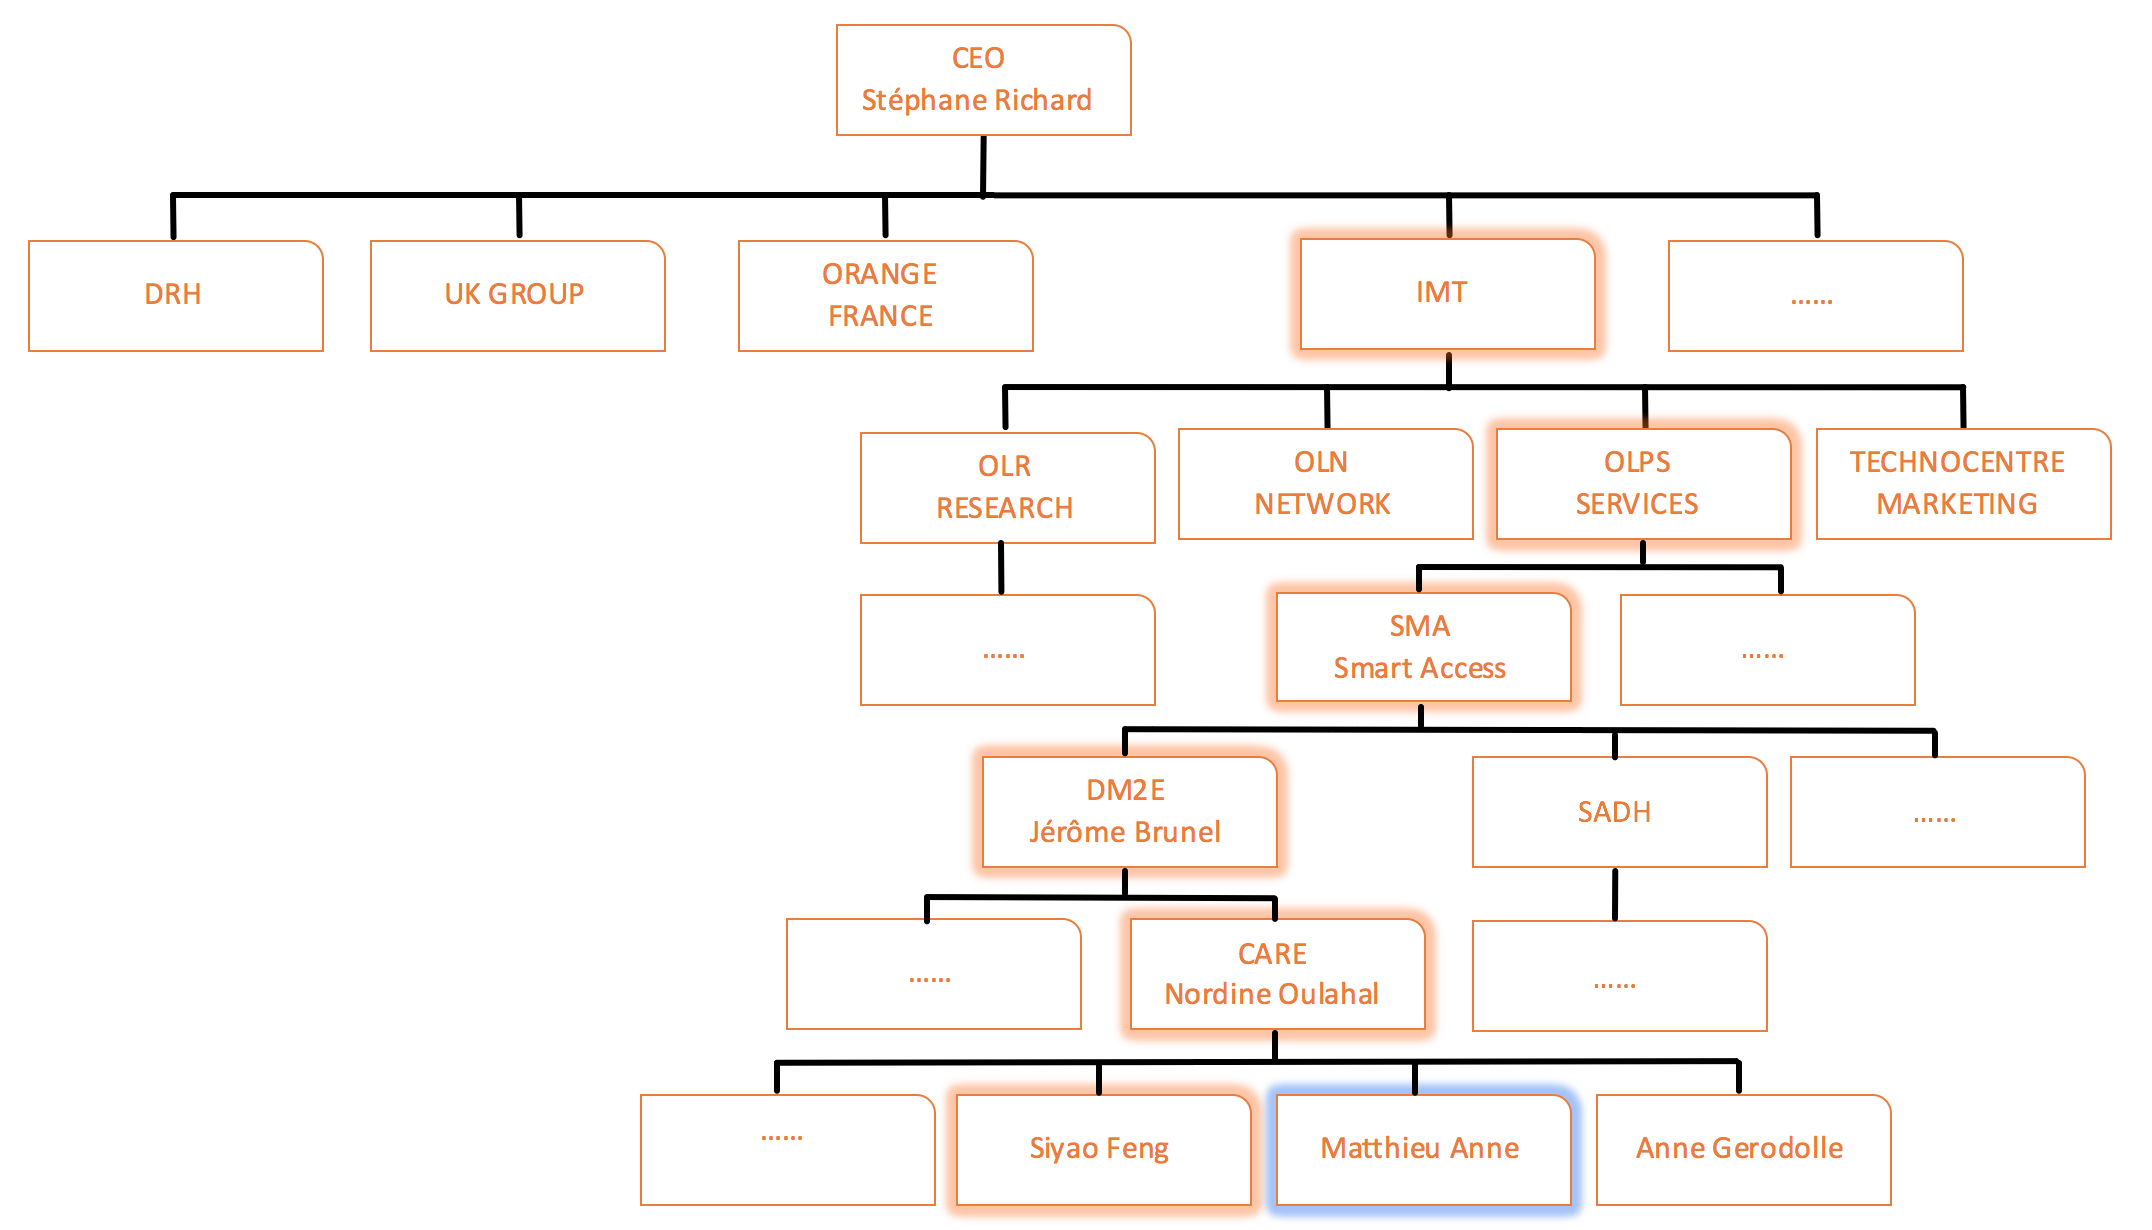
\includegraphics[width=15cm]{Figures/orgadiagramme.png}
	\caption[Partial flow chart showing the structure of Orange]{Partial flow chart showing the structure of Orange}
	\label{fig:structure}
\end{figure}
%----------------------------------------------------------------------------------------
\section{Team CARE}

I was integrated in the team CARE during my internship, which is for \textit{Cloud enablers for Administration of Residential Equipment}, the main purpose are:
\begin{itemize}
	\item Promote a consistent technical strategy between Tools and Devices on ``I need help'' process,
	\item Improve Orange customer satisfaction and reduce the cost of Broadband Services operation.
\end{itemize}

The Scope of ``CARE'' technical domain are:
\begin{itemize}
	\item Broadband Services
	\begin{itemize}
		\item Expertise and management of in-life Home Devices problems and bugs fixing with manufacturers
		\item Delivery and generalization of Home Devices corrective and functional( enhanced) versions
		\item Development of Home Devices diagnostic tools for Orange shops and for Customers
	\end{itemize}
	\item Mobile Services
	\begin{itemize}
		\item Collect, monitor and measure Mobile network quality and services(Qualimetre, CEM/CBM)
	\end{itemize}
\end{itemize}
%----------------------------------------------------------------------------------------

% Chapter 3

\chapter{Background} % Main chapter title here

\label{Chapter3} % For referencing the chapter elsewhere, use \ref{Chapter3}

\lhead{Chapter 3. \emph{Background}} % This is for the header on each page perhaps a shortened title


\definecolor{mygreen}{rgb}{0,0.6,0}
\definecolor{mygray}{rgb}{0.9,0.9,0.9}
\definecolor{mymauve}{rgb}{0.58,0,0.82}
\definecolor{mybrown}{RGB}{178,34,34}

%\frametitle{Inserting source code without setting typewriter}
\lstset{language=C++,
  backgroundcolor=\color{mygray},
  numbers=left,                    % possible val ues are (none, left, right)
  numbersep=-8pt,                   % how far the line-numbers are from the code
  numberstyle=\tiny\color{mybrown}, % the style that is used for the line-numbers
  stepnumber=1,                    % each line will be numbered
  morekeywords={*},
  keywordstyle=\color{blue},
  stringstyle=\color{mymauve},
  commentstyle=\color{mygreen},
  morecomment=[l][\color{magenta}]{\#},
  basicstyle=\footnotesize,        % the size of the fonts that are used for the code
  keepspaces=false,                 % keeps spaces in text, useful for keeping indentation of code
  columns=flexible,
  breaklines=true
  rulesepcolor=\color{mygray},
  rulecolor=\color{mygray}
}
%----------------------------------------------------------------------------------------
In this chapter, some important technical backgrounds will be covered. First it explains the \textit{CPE WAN Management Protocol (CWMP)} which defines several data models. Then is the Mios which is the main partner of Orange on the Smart Home project. Also the \textit{NAT traversal} will be presented after Mios, it is a computer networking methodology with the goal to establish and maintain Internet protocol connections across gateways that implement \textit{network address translation (NAT)}.At last, the Homelive box will be analysed, including the HardWare analyse, operating system OpenWRT and Cross-Compiling between working machine and the embedeed system OpenWRT.

\section{CWMP}

CPE WAN Management Protocol (CWMP) is a technology specification initiated and developed by the Digital Subscriber’s Line DSL Forum(now Broadband Forum). CWMP is numbered TR-069 by the forum and is thus also called the TR-069 protocol. It defines the general frame, message format, management method, and data model for the management and configuration of home network devices in next-generation networks.

CWMP is mainly applied to DSL access networks, which are hard to manage because user devices are located at the customer premise, dispersed, and large in number. CWMP makes the management easier by using an auto-configuration server (ACS) to perform remote centralized management of customer premises equipment (CPE).



\subsection{CWMP Protocol}
\label{basics}
CWMP is a text based protocol. Orders sent between the device (CPE) and auto configuration server (ACS) are transported over HTTP (or more frequently HTTPS)(\fref{fig:remotecontrol}). At this level (HTTP) CPE is behaving in the role of client and ACS in the role of HTTP server. This essentially means that control over the flow of the provisioning session is the sole responsibility of the device.
\begin{figure}[htbp]
	\centering
		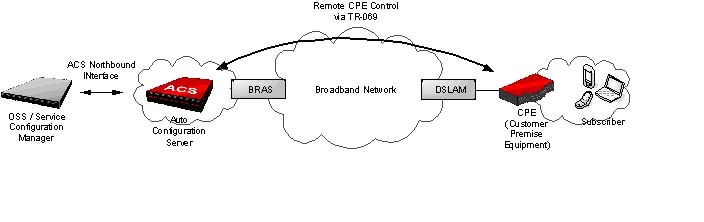
\includegraphics[width=9.5cm]{Figures/Remote_CPE_Control_via_TR-069.jpg}
	\caption[Remote CPE Control via TR-069]{Remote CPE Control via TR-069}
	\label{fig:remotecontrol}
\end{figure}
%-------------------------------------------------------
\subsubsection{Provisioning session}
All communications and operations are performed in the scope of the provisioning session. The session is always started by the device(CPE) and begins with the transmission of an Inform message. Its reception and readiness of the server for the session is indicated by an InformResponse message. That concludes the session initialization stage. The order of the next two stages depends on the value of the flag HoldRequests. If the value is false the initialization stage is followed by the transmission of device requests, otherwise ACS orders are transmitted first. The following description assumes the value is false.

In the second stage, orders are transmitted from the device to the ACS. Even though the protocol defines multiple methods that may be invoked by the device on the ACS, only one is commonly found - TransferComplete which is used to inform the ACS of the completion of a file transfer previously issued Download or Upload request. This stage is finalized by transmission of empty HTTP-request to the ACS.

In the third stage the roles change on the CWMP level. The HTTP-response for the empty HTTP-request by the device will contain a CWMP-request from the ACS. This will subsequently be followed by an HTTP-request containing a CWMP-response for the previous CWMP-request. Multiple orders may be transmitted one-by-one. This stage (and the whole provisioning session) is terminated by an empty HTTP-response from the ACS indicating that no more orders are pending.



\subsubsection{Security and authentication}
As vital data (like user names and passwords) may be transmitted to CPE via CWMP, it is essential to provide secure transport channel and always authenticate the CPE against the ACS. Secure transport and authentication of the ACS identity can easily be provided by usage of HTTPS and verification of ACS certificate. Authentication of the CPE is more problematic. The identity of the device is verified based on a shared secret (password) at the HTTP level. Passwords may be negotiated between the parties (CPE-ACS) at every provisioning session. When the device contacts the ACS for the first time (or after a factory-reset) default passwords are used. In large networks it is the responsibility of the procurement to ensure each device is using unique credentials, their list is delivered with the devices themselves and secured.


\subsubsection{Connection request}

The following example\fref{fig:connectionrequest} illustrates how CWMP works. The scenario: There are two ACSs, active and standby in an area. The active ACS needs to restart for system upgrade. To ensure a continuous monitoring of the CPE, the active ACS needs to let all the CPE in the area connect to the standby ACS. The whole process is as follows:

\begin{figure}[htbp]
	\centering
		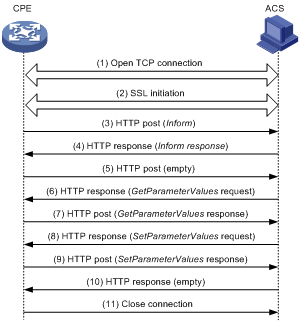
\includegraphics[width=9.5cm]{Figures/connection_request.png}
	\caption[CWMP Connection Scenario]{CWMP Connection Scenario}
	\label{fig:connectionrequest}
\end{figure}

\begin{enumerate}
  \item Establish a TCP connection
  \item SSL initiation, and establish a security mechanism
  \item The CPE sends an Inform request message to initiate a CWMP connection. The Inform message carries the reason for sending this message in the Eventcode field. In this example, the reason is “6 CONNECTION REQUEST”, indicating that the ACS requires the CPE to establish a connection.
  \item If the CPE passes the authentication of the ACS, the ACS returns an Inform response, and the connection is established.
  \item Receiving the Inform response, the CPE sends an empty message if it has no other requests. The CPE does this in order to comply with the request/reply interaction model of HTTP, in which CWMP messages are conveyed.
  \item The ACS queries the value of the ACS URL set on the CPE.
  \item The CPE replies the ACS with the obtained value of the ACS URL.
  \item The ACS finds that its local URL value is the same as the value of the ACS URL on the CPE. Therefore, the ACS sends a Set request to the CPE to modify the ACS URL value of the CPE as the URL of the standby ACS.
  \item The setting succeeds and the CPE sends a response.
  \item The ACS sends an empty message to notify the CPE that it has no other requests.
  \item The CPE closes the connection.
\end{enumerate}

After this, the CPE will initiate a connection to the standby ACS.

\subsubsection{CR over NAT}
The CWMP protocol also defines a mechanism for reaching the devices that are connected behind NAT (e.g. IP-Phones, Set-top boxes). This mechanism, based on STUN and UDP NAT traversal, is defined in document TR-069 Annex G (formerly in TR-111).

Amendment 5 of the protocol introduces alternative method of executing Connection Request via NAT based on XMPP (see Annex K of TR-069 Amendment 5 for details).


\subsection{Data Model}
The Broadband Forum defines several data models for use with the CPE WAN Management Protocol (TR-069 Amendment 5). These data models contain objects and parameters that describe the many different functions and capabilities available to devices and services that are manageable via CWMP.

CWMP data models are divided into two types: Root and Service. The root data model, Device1, is used to describe the major functions of a network aware device, including interfaces, software/firmware, diagnostics, components common to CWMP and other services, and the basic device information necessary to CWMP.

Service data models describe modular functionality that allow the extension of the root data model on a device (under Device.Services.) to provide particular services, such as a voice service, set top box service, network attached storage, etc.

Each data model is defined by a Name:Version syntax. A device defines its data model by defining a device type, an XML document that maps to (imports) BBF official data model objects and/or vendor specific objects. A full explanation of how to develop compliant CWMP data models can be found in TR-154.

%--------------------------------------
Most of the configuration and diagnostics is performed through setting and retrieving the value of the device parameters. These are organized in a well defined hierarchical structure that is more or less common to all device models and manufacturers. Broadband Forum publishes its data model standards in two formats - XML files containing a detailed specification of each subsequent data model and all of the changes between their versions and PDF files containing human-readable details. Supported standards and extensions should be clearly marked in the device data model. This should be in the field Device.DeviceSummary or InternetGatewayDevice.DeviceSummary which is required starting from Device:1.0 and InternetGatewayDevice:1.1 respectively. If the field is not found InternetGatewayDevice:1.0 is implied. As of Device:1.4 and InternetGatewayDevice:1.6 new field ( \'<RO>\'.SupportedDatamodel) for supported standard specification was introduced.

The model is always rooted in the single key named Device or InternetGatewayDevice depending on the manufacturer's choice. At each level of the structure objects and parameters (or array-instances) are allowed. Keys are constructed by concatenating the names of objects and parameter using '.'(dot) as a separator, e.g. InternetGatewayDevice.Time.NTPServer1 .

Each of the parameters may be marked as writable or non-writable. This is reported by the device in GetParameterNamesResponse message. The device should not permit the change of any parameter marked as read-only. Data model specifications and extensions clearly mark required status of most of the parameters.

Values applicable for the parameter, their type and meaning are also precisely defined by the standard.

\textbf{Multi-instance objects} :Some parts of the data model require the existence of multiple copies of the subtree. The best examples are those describing tables, e.g. Port Forwarding Table. An object representing an array will only have instance numbers or alias names as its children.

A multi-instance object may be writable (enabling dynamic creation and/or removal of its children) or read-only depending on the data represented. If for example the object represents four physical ports on a switch it should not be possible to add or remove them from the data model. If an instance is added to an object an identifier is assigned. After being assigned, identifiers may not change during the life-cycle of the device except for factory-reset.
%------------------------------------------------------------------------------------------------------------
\section{Mios}
MiOS, LTD. is a global software and hardware company represented in over 60 countries, and focused on developing and distributing advanced control and monitoring solutions for the home and small enterprise markets. Founded in 2008, MiOS has created the technology platform that bridges many different devices to produce hardware and software solutions for home control networks. Now in its fifth generation, the MiOS platform allows users to remotely control, monitor and automate their households and businesses with products that are currently available from any vendor.

At January 6th, 2014. MiOS has been selected as the platform partner for Orange’s Smart Home initiative. This announcement followed a successful launch with MiOS as the platform for Orange Poland’s Smart Home program.  The Orange initiative will be initially offered in several countries in Europe.

\subsection{Luup}
Luup (Lua-UPnP) is Mi Casa Verde(Mios)’s new software engine which incorporates \textit{Lua}, a popular scripting language, and \textit{UPnP}, the industry standard way to control devices. Vera is built on Luup.

On this platform, since the API includes drivers for Z-Wave, Insteon, etc., and talks to infrared and serial devices, home automation is the first thing that we can do on Luup. However Lua is a full-featured language and not limited just to scripting. Also, we can write modules in C/C++ that run on Vera, which the main Luup engine will also aggregate and control.

\subsection{MMS}
MMS is the management platform based on http request. To be able to use the MMS, we have to authenticate to a valid user of an account:

Here is a login example:
\begin{lstlisting}[mathescape]
	https://orangefut-autha1.com/autha/auth/username/bob?SHA1Password=86e739edcc&PK_Oem=33
\end{lstlisting}

And the body of the response (Identity and IdentitySignature are truncated):

\begin{lstlisting}[mathescape]
{
  "Identity": "eyJFeHBpcmVzIjoxNDAw...YW5nZV9tYXN0ZXIifQ==",
  "IdentitySignature": "L5H6babTjsZwk7RiAeRP...W91tWSMIbI9x7jJmsQ==",
  "Server_Event": "orangefut-event12.com",
  "Server_Event_Alt": "orangefut-event11.com",
  "Server_Account": "orangefut-account12.com",
  "Server_Account_Alt": "orangefut-account11.com"
}
\end{lstlisting}
%----------------------------------------------------------------------------------------------------------------
\section{NAT Traversal}
NAT traversal is a computer networking methodology with the goal to establish and maintain Internet protocol connections across gateways that implement network address translation (NAT). NAT breaks the principle of end-to-end connectivity originally envisioned in the design of the Internet.

NAT traversal techniques are required for certain client-to-client network applications, such as peer-to-peer file sharing and Voice over IP.\cite{stiemerling2008nat}

%----------------------------------------------------------------------------------------------------------------

\subsection{Principals}

Many techniques exist, but no single method works in every situation since NAT behavior is not standardized. Many NAT traversal techniques require assistance from a server at a publicly routable IP address\cite{rosenberg2003stun}. Some methods use the server only when establishing the connection, while others are based on relaying all data through it, which adds bandwidth costs and increases latency, detrimental to real-time voice and video communications.

NAT devices are commonly used to alleviate IPv4 address exhaustion\cite{alqahtaniipv4} by allowing the use of private IP addresses on home and corporate networks behind routers with a single public IP address facing the public Internet. The internal network devices communicate with hosts on the external network by changing the source address of outgoing requests to that of the NAT device and relaying replies back to the originating device.

The NAT traversal techniques available are as following:
\begin{itemize}
  \item \textit{Socket Secure (SOCKS)} is a technology created in the early 1990s that uses proxy servers to relay traffic between networks or systems.
  \item \textit{UPnP IGD} is supported by many small NAT gateways in home or small office settings.
  \item \textit{Interactive Connectivity Establishment (ICE)} is a technique used in VoIP, peer-to-peer communications, video, instant messaging, and other interactive media applications. It uses Session Traversal Utilities for NAT (STUN).
  \item \textit{Application-level gateway (ALG)} is a component of a firewall or NAT that allows for configuring NAT traversal filters.\cite{hu2005nat}
  \item \textit{NAT hole punching} is a technique that exploits how NATs handle some protocols (for example, UDP, TCP, or ICMP) to allow previously blocked packets through the NAT.
\end{itemize}

At Orange Labs, we use \textit{UPnP IGD} and \textit{STUN}to manage NAT traversal.
%----------------------------------------------------------------------------------------------------------------
\subsection{UPnP IGD}

Universal Plug and Play (UPnP)\cite{jeronimo2003upnp} is a set of networking protocols that permits networked devices, such as personal computers, printers, Internet gateways, Wi-Fi access points and mobile devices to seamlessly discover each other's presence on the network and establish functional network services for data sharing, communications, and entertainment. UPnP is intended primarily for residential networks without enterprise-class devices.

The UPnP technology is promoted by the UPnP Forum, a computer industry initiative to enable simple and robust connectivity to stand-alone devices and personal computers from many different vendors. The Forum consists of over eight hundred vendors involved in everything from consumer electronics to network computing.

The concept of UPnP is an extension of plug-and-play, a technology for dynamically attaching devices directly to a computer, although UPnP is not directly related to the earlier plug-and-play technology. UPnP devices are "plug-and-play" in that when connected to a network they automatically establish working configurations with other devices.

Internet Gateway Device (IGD) Standardized Device Control Protocol is a protocol for mapping ports in network address translation (NAT) setups, supported by a certain number of NAT-enabled routers.\cite{wing2013p} It is a common communications protocol of automatically configuring port forwarding, and is part of an ISO/IEC Standard \cite{sherwin2009upnp} rather than an Internet Engineering Task Force standard.

Applications using peer-to-peer networks, multiplayer gaming, and remote assistance programs need a way to communicate through home and business gateways. Without IGD one has to manually configure the gateway to allow traffic through, a process which is error prone and time consuming. Universal Plug and Play (UPnP) comes with a solution for network address translation traversal.

IGD makes it easy to do the following:

\begin{itemize}
  \item Learn the public (external) IP address
  \item Requesting for a new public IP address\cite{srisuresh1999ip}
  \item Enumerate existing port mappings
  \item Add and remove port mappings
  \item Assign lease times to mappings
\end{itemize}
%----------------------------------------------------------------------------------------------------------------
\subsection{STUN}
STUN (Session Traversal Utilities for NAT) is a standardized set of methods and a network protocol to allow an end host to discover its public IP address if it is located behind a NAT. It is used to permit NAT traversal for applications of real-time voice, video, messaging, and other interactive IP communications. It is documented in RFC 5389\cite{rosenberg2008rfc}. The STUN URI scheme is documented in RFC 7064. STUN is intended to be a tool to be used by other protocols, such as ICE.

The STUN protocol allows applications operating behind a network address translator (NAT) to discover the presence of the network address translator and to obtain the mapped (public) IP address (NAT address) and port number that the NAT has allocated for the application's User Datagram Protocol (UDP) connections to remote hosts. The protocol requires assistance from a third-party network server (STUN server) located on the opposing (public) side of the NAT, usually the public Internet.


\begin{figure}[htbp]
	\centering
		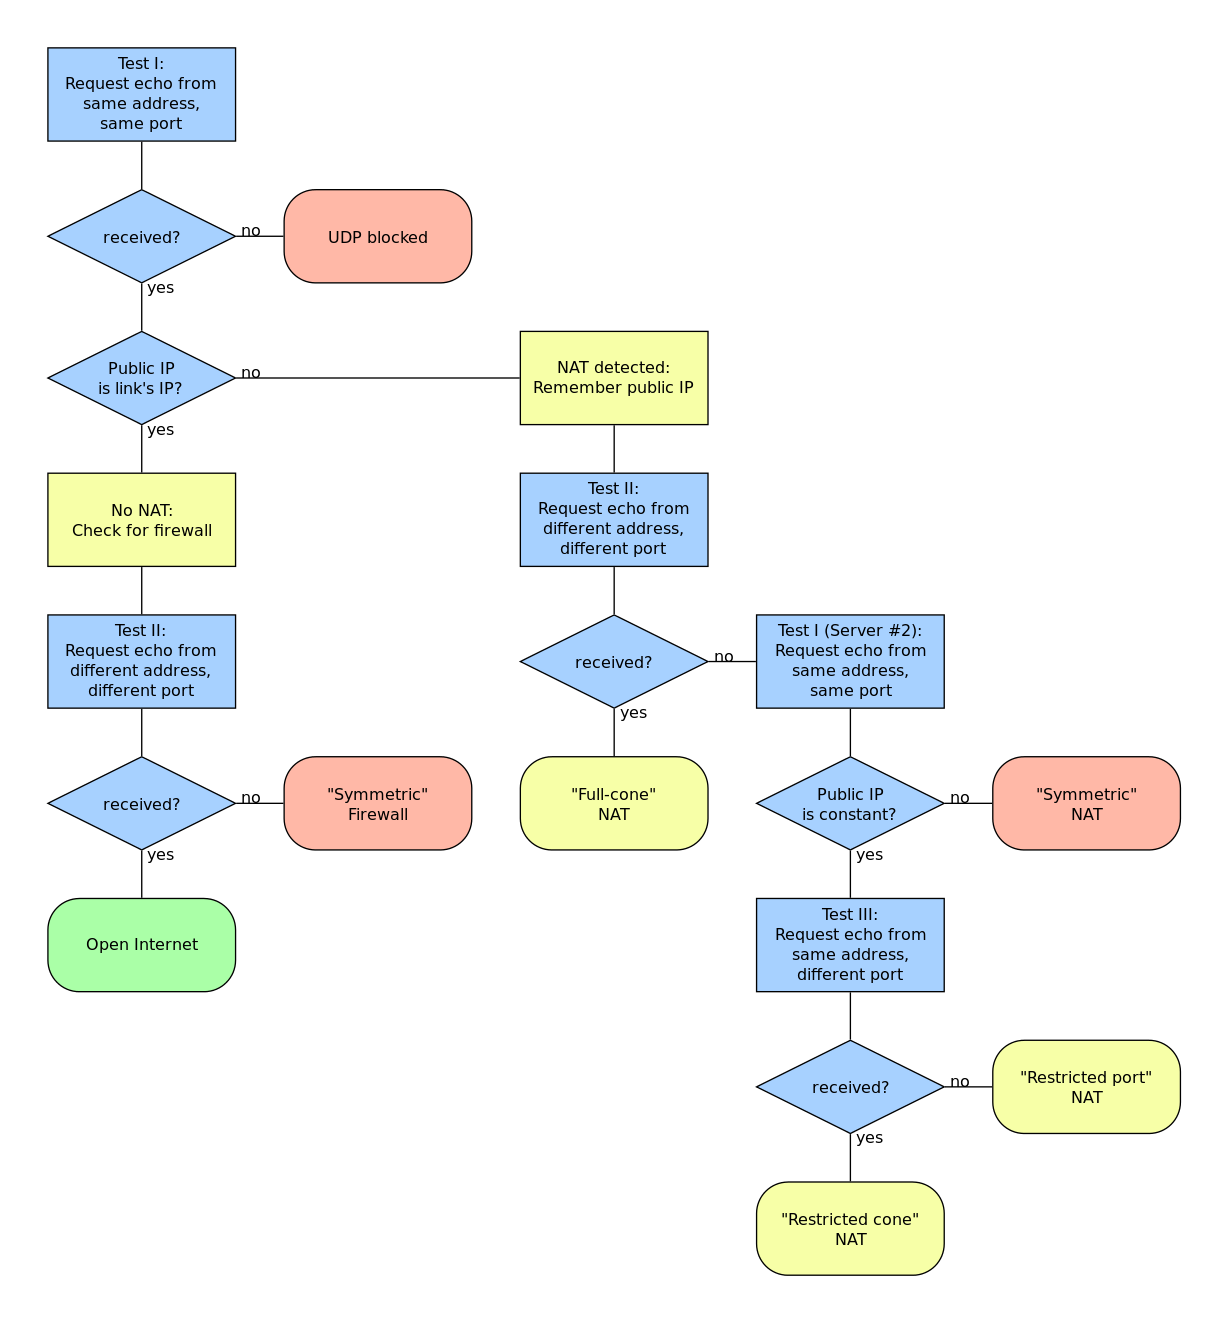
\includegraphics[width=9.5cm]{Figures/STUN_Algorithm.png}
	\caption[STUN Algorithm to track the Public Address]{STUN Algorithm to track the Public Address}
	\label{fig:stunalgorithm}
\end{figure}
%----------------------------------------------------------------------------------------------------------------
\section{Homelive Box}
Homelive is the Smart Home set-top box of Orange, which is the center of the Z-Wave network.

%----------------------------------------------------------------------------------------------------------------
\subsection{Hardware}

\begin{figure}[htbp]
	\centering
		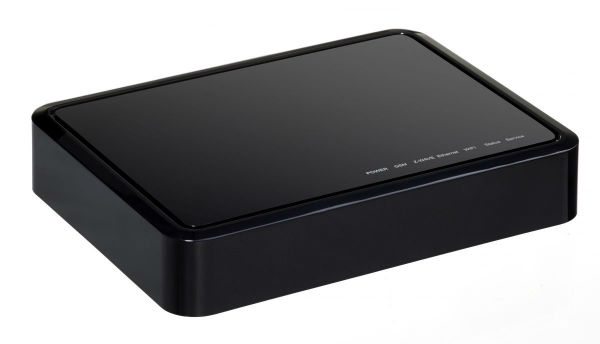
\includegraphics[width=9.5cm]{Figures/Orange-Home-Live.jpg}
	\caption[Homelive Box of Orange]{Homelive Box of Orange}
	\label{fig:homelivebox}
\end{figure}

Here is the list of Homelive components:

\begin{center}
  \begin{tabular}{@{} cc @{}}
    \toprule
    Item & Value \\*
    \midrule
    Architecture & MIPS64 \\
    Operating System & OpenWRT BarrierBreaker 14.07\\
    Firmware & Luup (Lua \& UPnP) \\
		Processeur & MT7620A (580 MHz) \\
		Capacité mémoire & 128 MB DDR2, 128 MB capacité flash NAND \\
		Connectivité Cellulaire & 2G quad bandes \\
		Connectivité RF & Z-Wave Serie 500 \\
		Connectivité Wi-Fi & 2.4 GHz 11n 2x2 \\
		Connectivité réseau & 1 port RJ45 10/100 \\
		Connectivité multimédia & 1 port USB2.0 \\
		Carte Sim & 1 Slot externe \\
		Dimensions & 174 mm x 129 mm x 33 mm (L x l x h) \\
		Poids & 421 g \\
		Alimentation externe & 12 V \\
		Consommation électrique & 3 W \\
    \bottomrule
  \end{tabular}
%	\caption[Homelive Box of Orange]{Homelive Box of Orange}
\end{center}

The MIPS64 architecture is based on a fixed-length, regularly encoded instruction set, and it uses a load/store data model. It is streamlined to support optimized execution of high-level languages. Arithmetic and logic operations use a three-operand format, allowing compilers to optimize complex expressions formulation. Availability of 32 general-purpose registers enables compilers to further optimize code generation by keeping frequently accessed data in registers.
%----------------------------------------------------------------------------------------------------------------
\subsection{OpenWRT}
OpenWrt\cite{fainelli2008openwrt} is a highly extensible GNU/Linux distribution for embedded devices (typically wireless routers). Unlike many other distributions for these routers, OpenWrt is built from the ground up to be a full-featured, easily modifiable operating system for your router. In practice, this means that you can have all the features you need with none of the bloat, powered by a Linux kernel that's more recent than most other distributions. The main components are the Linux kernel, util-linux, uClibc or musl, and BusyBox. All components have been optimized for size, to be small enough for fitting into the limited storage and memory available in home routers.

OpenWrt is configured\cite{petullo2010building} using a command-line interface (ash shell), or a web interface (LuCI). There are about 3500 optional software packages available for installation via the opkg package management system.

OpenWrt can run on various types of devices, including \textit{CPE routers}, residential gateways, smartphones (e.g. Neo FreeRunner), pocket computers (e.g. Ben NanoNote), and laptops (e.g. One Laptop per Child (OLPC)). It is also possible to run OpenWrt on ordinary computers, which are most commonly based on the x86 architecture. Many patches from the OpenWrt's codebase have been included upstream in the Linux kernel mainline.
%----------------------------------------------------------------------------------------------------------------
\subsection{Cross-Compiling}

Cross compiling is the process that capable of creating executable code for a platform other than the one on which the compiler is running. For example, a compiler that runs on a Windows 7 PC but generates code that runs on Android smartphone is a cross compiler.

In our case, in the reason of the source of hardware in Homelive is very limited, we should finish the compilation of source code under the Linux Machine. To archieve this, we should get prepared with the compile tool chain which is provided by OpenWRT. The steps are:

\begin{enumerate}
  \item Download OpenWRT package prom officail site
  \item Compile OpenWRT on Linux machine and select the packages needed for Homelive Box
  \item Generate the tool-chain of compilation
  \item Comple the TR-069 source code with OpenWRT tool chain
  \item Transfer excutable files to Homelive
\end{enumerate}

The disadvantage of cross compiling is that we can\'t use debug tools like \textit{GDB}.

% Chapter 4

\chapter{HomeLive Management Platform} % Main chapter title

\label{Chapter4} % For referencing the chapter elsewhere, use \ref{Chapter4}

\lhead{Chapter 4. \emph{HomeLive Management Platform}} % This is for the header on each page - perhaps a shortened title

%----------------------------------------------------------------------------------------
In this chapter, the Homelive Management Platform structure will be introduced. The following figure shows an overview for the application between ACS and CPE
devices. With TR-069 protocol, ACS can communicate and manage devices easily. 
%http://orange-france.com.francetelecom.fr:81/ui_normandie/spip.php?article3304
\begin{figure}[htbp]
	\centering
		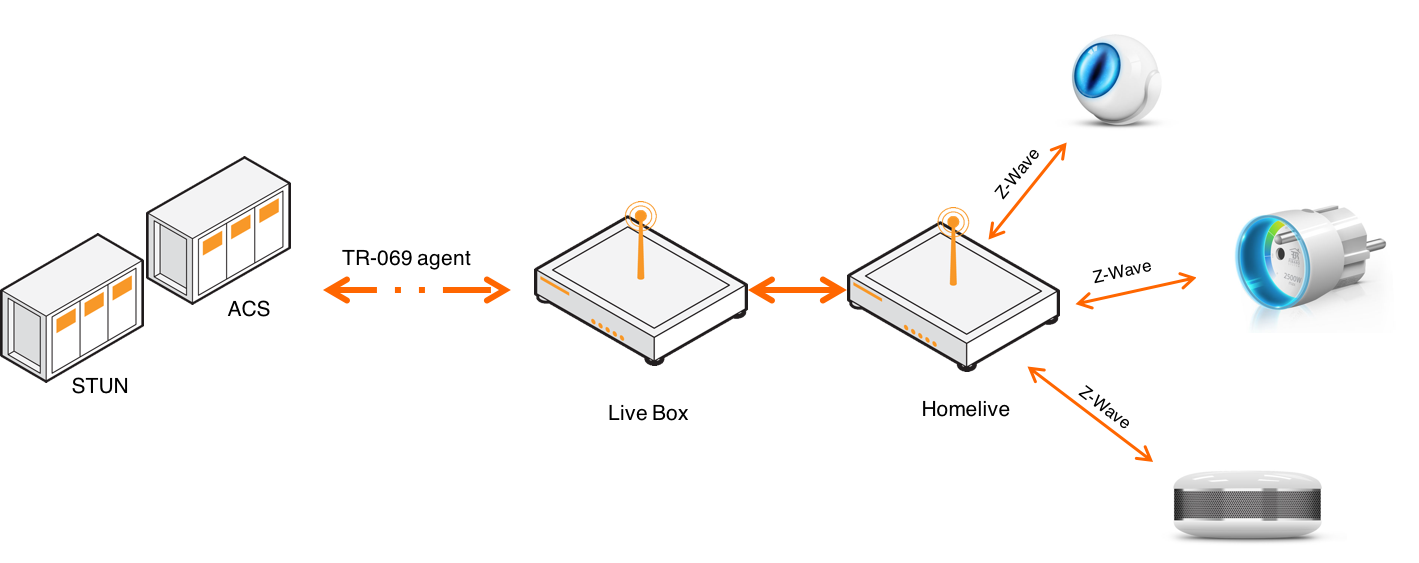
\includegraphics[width=9.5cm]{Figures/Homelive_Management_Platform.png}
	\caption[Homelive Management Platform]{Homelive Management Platform}
	\label{fig:Platform}
\end{figure}

ACS is the server which is accessible by the support engineers of Orange. Support engineers can communicate at distance with Homelive box using protocol TR-069. The TR-069 server will be running in ACS and TR-069 client will be running in Homelive. This essentially means that control over the flow of the provisioning session is the sole responsibility of the device. Through TR-069, the high-level operations possible are:
\begin{itemize}
  \item Service activation and reconfiguration
  \begin{itemize}
    \item Initial configuration of the service as part of zero-touch or one-touch configuration process
    \item Service re-establishment (ex. after device is factory-reset, exchanged)
  \end{itemize}
  \item Remote Subscriber Support
  \begin{itemize}
    \item Verification of the device status and functionality
    \item Manual reconfiguration
  \end{itemize}
  \item Firmware and Configuration Management
  \begin{itemize}
    \item Firmware upgrade/downgrade
    \item Configuration backup/restore
  \end{itemize}
  \item Diagnostics and monitoring
  \begin{itemize}
    \item Throughput (TR-143) and connectivity diagnostics
    \item Parameter value retrieval
    \item Log file retrieval
  \end{itemize}
\end{itemize}
%----------------------------------------------------------------------------------------------------------------------
\section{Auto Configuration Server}

% Chapter 5

\chapter{TR-069 Client} % Main chapter title

\label{Chapter5} % For referencing the chapter elsewhere, use \ref{Chapter5}

\lhead{Chapter 5. \emph{TR-069 Client}} % This is for the header on each page - perhaps a shortened title

\lstdefinestyle{DOS}
{
    backgroundcolor=\color{black},
    basicstyle=\scriptsize\color{white}\ttfamily
    numbers=none,
    numbersep=8pt,                   % how far the line-numbers are from the code
    numberstyle=\tiny\color{white}, % the style that is used for the line-numbers
    stepnumber=1                    % the step between two line-numbers. If it's 1, each line will be numbered
}
%----------------------------------------------------------------------------------------
\lstdefinestyle{C}
{
  morekeywords={export}
}
%----------------------------------------------------------------------------------------
TR-069 Client is implemented by Orange at 2008, but is a generic version for all potential devices. The first part of my internship is to make TR-069 Client for Homelive Box. To be able to provide a generic TR-069 module which is easily portable on different devices, it satisfy the following points:

\begin{itemize}
  \item Written in ANSI C
  \item Small memory footprint
  \item Provide generic API to access device specific modules
  \item Provide Makefiles to build the binary
  \item Provide system traces on module activity
\end{itemize}

On a CPE, there are two modules that are mentioned all along this document and which are responsible of
the CWMP:
\begin{itemize}
  \item \textbf{TR-069 Agent}: This agent is responsible of the CWMP sessions. It initializes them with the inform message, realizes the ACS command(s) and execute some feedback command (notably after a firmware upgrade).
  \item \textbf{TR-069 Server}: This is a small HTTP server which listens of the WAN interface for an ACS solicitation (in TR-069, it is known as “connection request”). On a valid connection request, the TR-069 server contacts the TR-069 agent for starting a CWMP session with the ACS.
\end{itemize}
%----------------------------------------------------------------------------------------
\section{Architecture of TR-069 Client}
The TR069 Generic Agent is composed of several modules and interfaces. Some modules are generic and can be ported with no modification. Other modules are platform specific (specific libraries usage, specific device API to get/set values, ...) and must implement services declared into generic interfaces.

\begin{figure}[htbp]
	\centering
		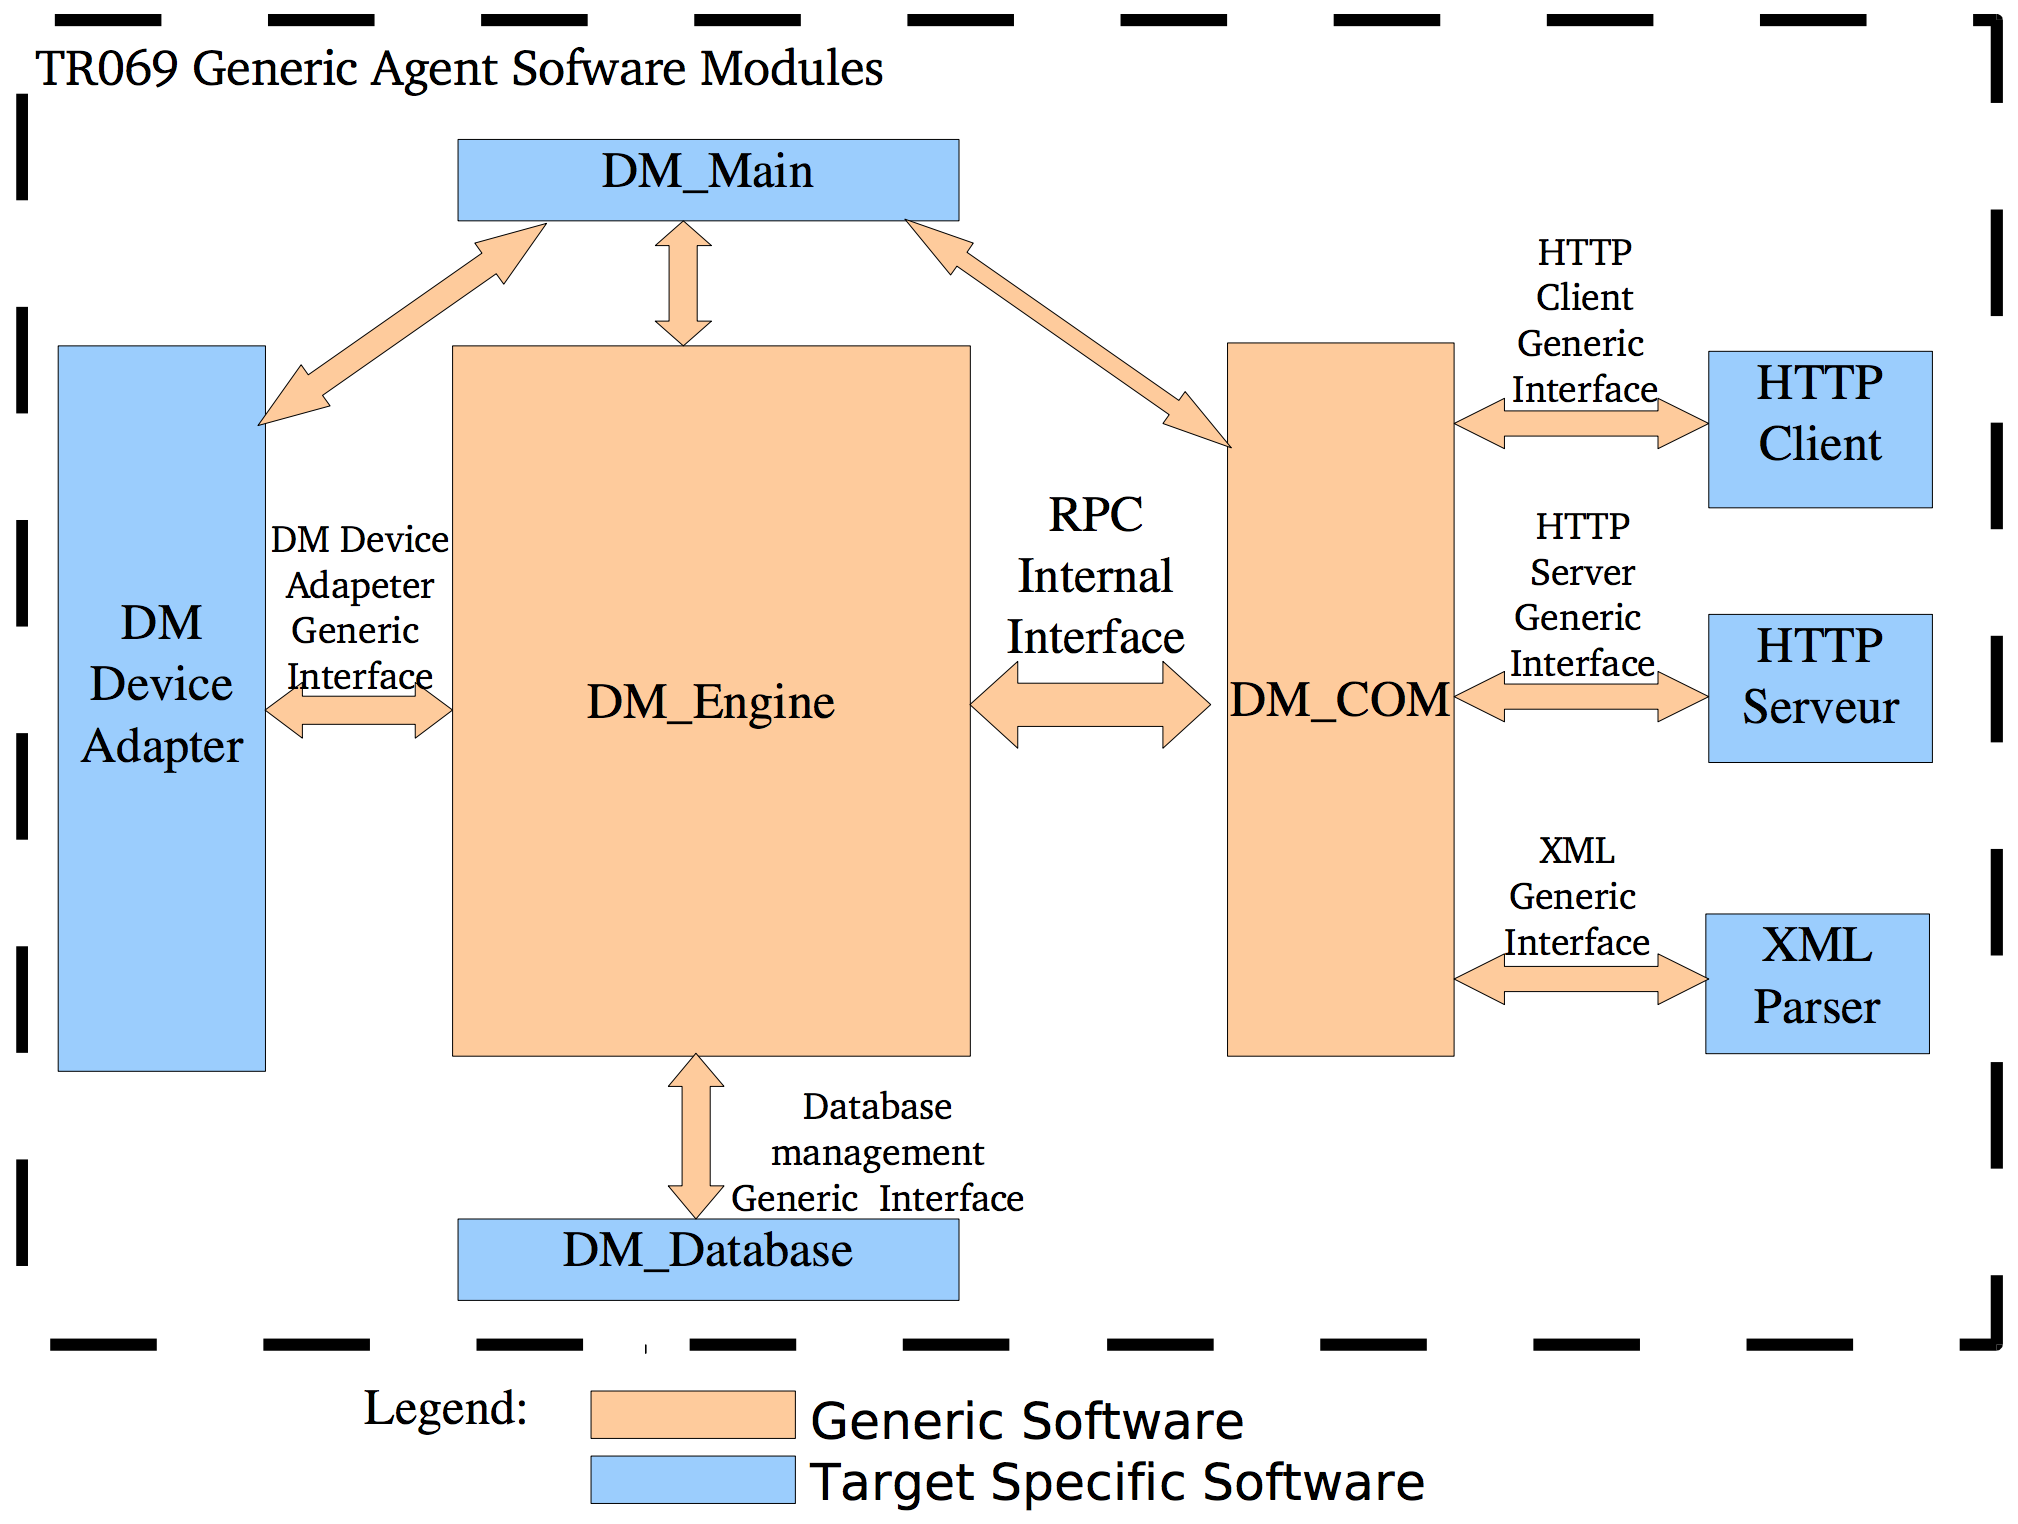
\includegraphics[width=12cm]{Figures/structuretr069.png}
	\caption[TR-069 Structure]{TR-069 Structure}
	\label{fig:tr069}
\end{figure}

For each module:
\begin{itemize}
  \item \textbf{DM\_ Engine} : In charge of the TR-069 logic,
  \item \textbf{DM\_ Com} : Handles the HTTP, SOAP and SSL Protocol with the ACS (Auto Configuration Server),
  \item \textbf{DM\_ DeviceAdapter} : Adaptation layer between the DM_Engine and the device system. It allows the implementation of the RPC commands (Get Parameter Value, Set Parameter Value, Reboot, Download, ...),
  \item \textbf{DM\_ Database} : Stores the data using an available storage solution on the device (or thanks to simple file storage),
  \item \textbf{HTTP Client} : Sets up / releases the HTTP connection with the ACS and sends / receives SOAP messages. The HTTP Client also handles SSL protocol,
  \item \textbf{HTTP SERVER} : Perform ACS Connection Request response,
  \item \textbf{XML Parser} : Decode / encode SOAP messages.
\end{itemize}

The figure below shows the file tree of the project, TR-069 Client defines all functions and APIs at each module. In consideration of easily ported to other devices, it put all target-related implementations in the folder \textit{dm\_target\_implementation}.

\begin{figure}[htbp]
	\centering
		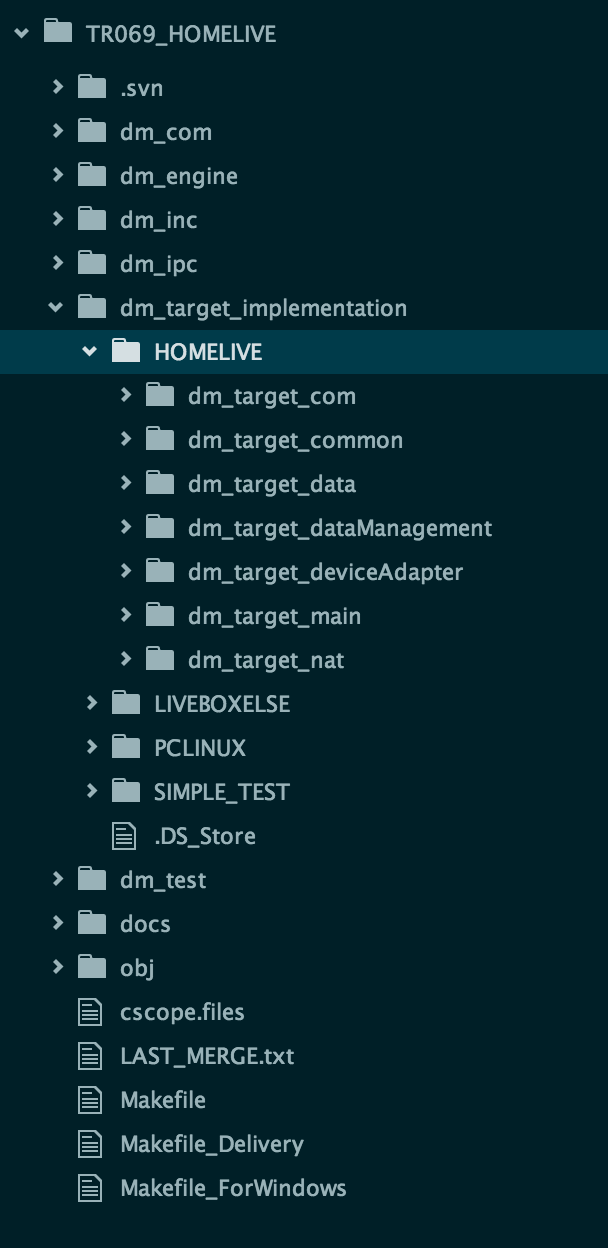
\includegraphics[width=8cm]{Figures/tr069_files.png}
	\caption[TR-069 File Tree Structure]{TR-069 File Tree Structure}
	\label{fig:tr069file}
\end{figure}

In the folder \textit{dm_taget_implementation}, different target has been defined, you can implement the APIs and Modules for different devices, and you specifie the target to compile in compilation, like:

\begin{lstlisting}[style=DOS][language=bash]
  $ make Target=TargetName TRACE_LEVEL=7 DEBUG=Y
  $ make clean Target=TargetName
\end{lstlisting}

A csv file must be created for each new platform. This CSV file describes the data model parameters used by TR069 Agent and the default values for the TR069 specifics parameters. This target dependent CSV file is stored into \\\textit{dm\_target\_implementation/MYNEWDEVICE/dm\_dm\_target\_data/dm\_csv} directory.

The CSV file is only read during the first system start up (or after a factory reset) and is used to generate the TR069
database (i.e. parameters.data and parameters.data\~{} files)

%----------------------------------------------------------------------------------------

\section{Problems and Solutions}

When ported the TR-069 Client to Homelive, we have encountered several problems before it can perfectly run on Homelive Box.

%----------------------------------------------------------------------------------------

\subsection{IP Address Error}
The first problem is IP Address Error. At every start up of the TR-069 Client, the module will have to detect the IP address of the box, and use it to build connection between STUN server and CPE. But when executing, the TR-069 client can't detect the IP address, so I have located the code which are responsible for IP detection,

\begin{lstlisting}[mathescape]
    static const char* ETH_INTERFACE = "eth0";
    struct ifaddrs *myaddrs = NULL, *ifa = NULL;
    struct sockaddr_in *s4 = NULL;
    int  status;
    /* but must be big enough for an IPv6 address (e.g. 3ffe:2fa0:1010:ca22:020a:95ff:fe8a:1cf8) */
    char buf[64];
    memset((void *) buf,  0x00, sizeof(buf));

    status = getifaddrs(&myaddrs);
    if (status == 0)
    {
       for (ifa = myaddrs; ifa != NULL; ifa = ifa->ifa_next)
       {
          if ( (ifa->ifa_addr != NULL)
             && ((ifa->ifa_flags & IFF_UP) != 0)
             && (ifa->ifa_addr->sa_family == AF_INET) )
          {
             s4 = (struct sockaddr_in *)(ifa->ifa_addr);
             if ( (inet_ntop(ifa->ifa_addr->sa_family, (void *)&(s4->sin_addr), buf, sizeof(buf)) != NULL)
                && (strcmp(ifa->ifa_name, ETH_INTERFACE)==0) )
             {
                ipAddress = strdup(buf);
                break;
             }
          }
       }
    }
\end{lstlisting}

In general, the first Internet address should be \textit{eth0}, but in Homelive Box, if you verify with command
\begin{lstlisting}[style=DOS][language=bash]
  $ ifconfig -a
\end{lstlisting}

The default Internet interface is "br-lan", which is specific in OpenWRT system, which is bridged Virtual Network Interface, used to make multiple virtual or physical network interfaces act as if they were just one network interface (quasi the opposite of VLANs).

So the solution is to change the macro definition of \textit{ETH\_INTERFACE} from \textit{``eth0''} to \textit{``br-lan''}. After the modification, the program can success finding the IP address.
%----------------------------------------------------------------------------------------
\subsection{STUN Initialization}

When using the default data model provided, TR-069 Client can't build connection with STUN server. By looking into the log file, the problem aims to no STUN data model has been settled. The solution is to add the items which describe STUN parameters as follow:
\begin{lstlisting}[mathescape]
    ManagementServer.UDPConnectionRequestAddress;STRING;0;0;1;2;1;0;;0;0;0
    ManagementServer.UDPConnectionRequestAddressNotificationLimit;UINT;0;1;0;0;0;0;;0;0;0
    ManagementServer.STUNEnable;BOOLEAN;0;1;0;0;1;0;;1;0;0
    ManagementServer.STUNServerAddress;STRING;0;1;0;0;1;0;;161.105.161.211;0;0
    ManagementServer.STUNServerPort;INT;0;1;0;0;1;0;;3478;0;0
    ManagementServer.STUNUsername;STRING;0;1;0;0;0;0;;test;0;0
    ManagementServer.STUNPassword;STRING;0;1;0;0;0;0;;1234;0;0
    ManagementServer.STUNMaximumKeepAlivePeriod;INT;0;1;0;0;0;0;;400;0;0
    ManagementServer.STUNMinimumKeepAlivePeriod;UINT;0;1;0;0;0;0;;10;0;0
    ManagementServer.NATDetected;BOOLEAN;0;0;1;2;1;0;;0;0;0
\end{lstlisting}
%----------------------------------------------------------------------------------------
\subsection{Memory Alignment Error}
After the modifications above, every time when running the TR-069 Client, after 2 seconds, the program crash and report \textit{bus error}, a bus error is a fault raised by hardware, notifying an operating system (OS) that a process is trying to access memory that the CPU cannot physically address: an invalid address for the address bus, hence the name. In modern use on most architectures these are much rarer than segmentation faults, which occur primarily due to memory access violations: problems in the logical address or permissions.

Because the TR-069 is generated by cross-compiling, some platforms (in our case MIPS64) can only read or write ints from addresses that are an even multiple of 8 bytes, otherwise they segfault. Even the ones that can handle arbitrary alignments are slower dealing with unaligned data (they have to fetch twice to get both halves), so the compiler will often pad structures to align variables. Treating structures as a lump of data that can be sent to disk or across the network thus requires extra work to ensure a consistent representation.

In the source code, there are \textit{struct} defined like:
\begin{lstlisting}[mathescape]
    typedef struct _DM_ENG_Parameter
    {
    	bool writable; //1 byte
    	char* name;  // 4 bytes
      int minValue; // 4 bytes

      ....

      struct _DM_ENG_Parameter* next;
    } __attribute((packed)) DM_ENG_Parameter;
\end{lstlisting}


In a 32bits processor, the first three elements of the structure will be aligned like \fref{fig:side:a}. But when using the attribute (packed), the memory will become \fref{fig:side:b} to save the memory space.

\begin{figure}
\begin{minipage}[t]{0.5\linewidth}
\centering
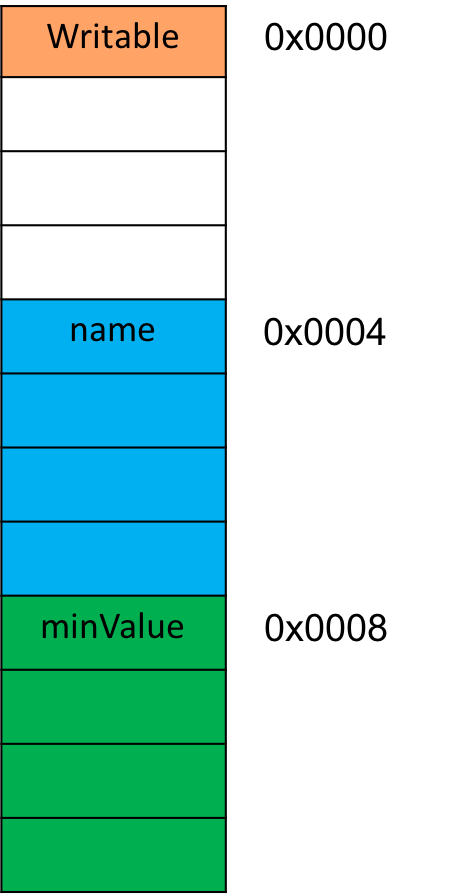
\includegraphics[width=4cm]{Figures/alignement1.png}
\caption{Memory Algnement under 32bits system}
\label{fig:side:a}
\end{minipage}%
\begin{minipage}[t]{0.5\linewidth}
\centering
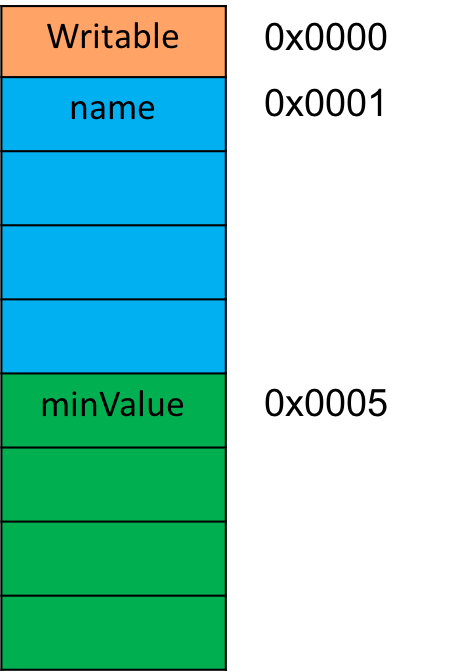
\includegraphics[width=4cm]{Figures/alignement2.png}
\caption{Memory Algnement under 32bits system with packed}
\label{fig:side:b}
\end{minipage}
\end{figure}


Under the Homelive architecture, it can only read data from address that is multiple of 4, so when the program tries to read value of name, the address is 0x0001 which is not an valid address, it reports the \textit{bus error}. To solve this bus error, the easiest way is to delete the attribute \textit{packed}, and then the compilator will automatic shift the address to meet the requirements.

%----------------------------------------------------------------------------------------
\section{RPC methods}
The next step is to verify and implement all the RPC methods, after verification:
\begin{center}
  \begin{tabular}{@{} cc @{}}
    \toprule
    RPC Method & Result \\*
    \midrule
    Connection Request & Yes \\
    Get RPC Methods & Yes \\
    Set Parameter Values  & Yes\\
    Get Parameter Values  & Yes\\
    Set Parameter Attributes  & Yes\\
    Get Parameter Attributes  & Yes\\
    Get Parameter Names & Yes\\
    Add Object  & Yes\\
    Delete Object & Yes\\
    Reboot & No\\
    Downloaded  & Yes\\
    Factory Reset & Yes\\
    Schedule Inform & Yes\\
    Upload & Yes\\
    \bottomrule
  \end{tabular}
%	\caption[Homelive Box of Orange]{Homelive Box of Orange}
\end{center}

When we call \textit{reboot} from ACS, the TR-069 turns out only reboot the program but not the whole box. To repair this, after located the reboot function, we added one line at the end of the function to let the program call the box to reboot after 5 seconds (which is for the TR-069 to shutdown all the process).
\begin{lstlisting}[mathescape]
  /*Reboot system after 5 seconds*/
  system("(sleep 5 && reboot) &");
\end{lstlisting}

% Chapter 6

\chapter{Z-Wave} % Main chapter title

\label{Chapter6} % For referencing the chapter elsewhere, use \ref{Chapter6}

\lhead{Chapter 6. \emph{Z-Wave}} % This is for the header on each page - perhaps a shortened title
Homelive use a new Smart Home communication technology -- Z-Wave. TR-069 Client should be able to retrieve the data in Luup and synchronize with TR-069 data model and ACS.

\begin{figure}[htbp]
	\centering
		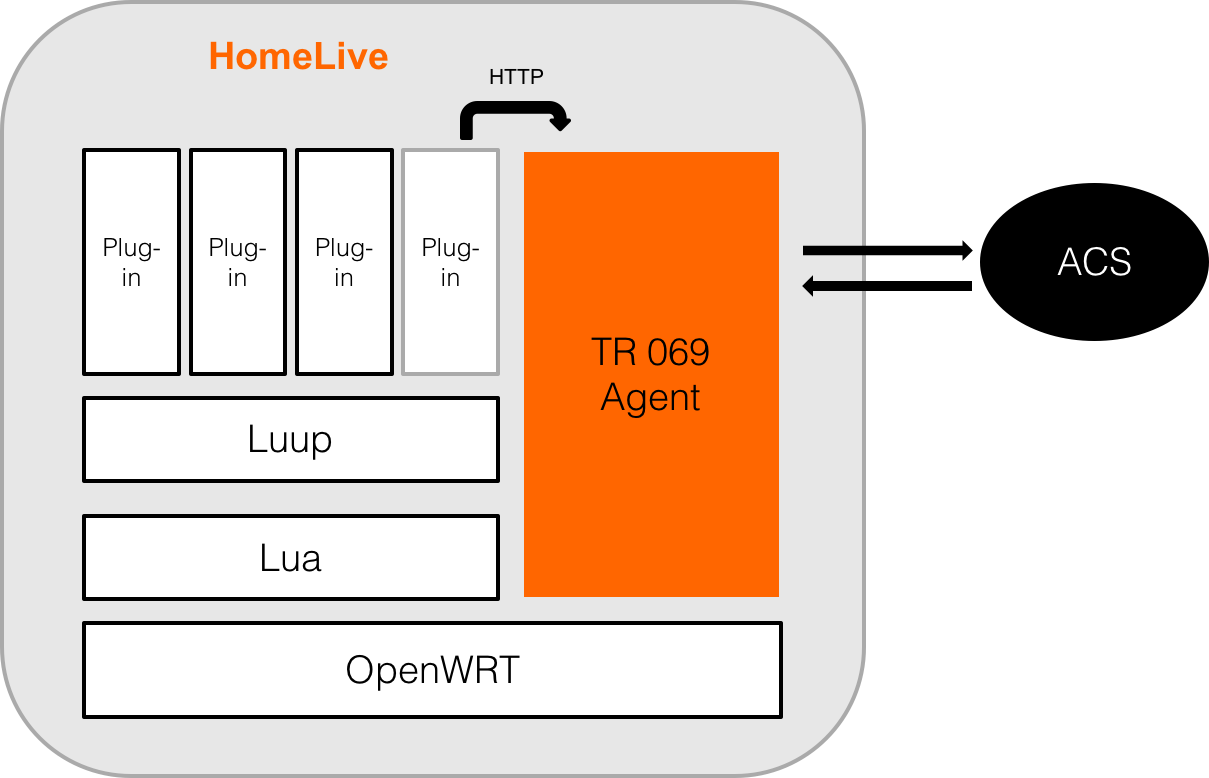
\includegraphics[width=12cm]{Figures/homelivestructure.png}
	\caption[Homelive Structure]{Homelive Structure}
	\label{fig:homelive}
\end{figure}

%----------------------------------------------------------------------------------------
\section{Protocol Z-Wave}
Z-Wave is a standardized protocol for automation wireless habitat solution. It was designed by the Danish company \textit{Zen-Sys} which was later bought by the US company \textit{Sigma Designs} in 2008. \textit{Sigma Designs} and the Japanese company Mitsumi provides the Z-Wave chips.

Z-Wave equipment manufacturers are gathered in the Z-Wave Alliance. Founded in 2005, it promotes the protocol and ensures interoperability between devices. Interoperability is true on two levels: Radio layer and application layer. Certified equipment receive the Z-Wave logo (see \fref{fig:zwavelogo}). More than three hundred companies have since joined this alliance.

\begin{figure}[htbp]
	\centering
		
\includegraphics[width=8cm]{Figures/zwavelogo.jpg}
	\caption[Z-Wave Protocol Logo]{Z-Wave Protocol Logo}
	\label{fig:zwavelogo}
\end{figure}

The Z-Wave radio protocol is optimized to communicate with low bandwidth (between 9 and 40 kbps) and applied on stand-alone power supply or mains-powered, as opposed to Wi-Fi, which is intended for exchanges broadband.

\begin{center}
  \begin{tabular}{@{} cccc @{}}
    \toprule
    Requirements\textbackslash Protocol & \textbf{Z-Wave} & \textbf{Zigbee} & \textbf{En-Ocean} \\*
    \midrule
    \textbf{Reliability} & Yes & Yes & No \\
    \textbf{Security} & Yes & Yes & No \\
    \textbf{Radio waves Reduction} & Yes & Yes & Yes \\
    \textbf{Simplicity of use} & Yes & - & No \\
    \textbf{Better pricing} & Not yet & Not yet & No \\
    \textbf{Capitalization} & Yes & - & Yes \\
    \textbf{Interoperability} & Yes & No & Yes \\
    \bottomrule
  \end{tabular}
%	\caption[Homelive Box of Orange]{Homelive Box of Orange}
\end{center}
\begin{figure}[htbp]
	\centering
		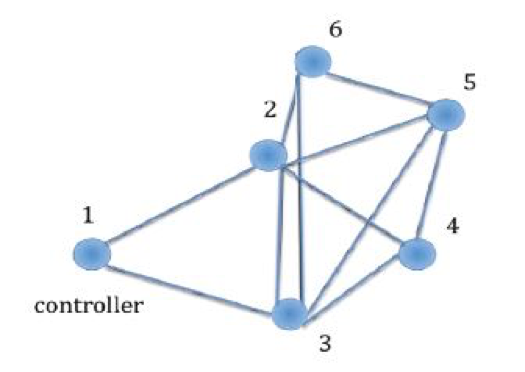
\includegraphics[width=8cm]{Figures/zwavenetwork.png}
	\caption[A Z-Wave Mesh Network Example]{A Z-Wave Mesh Network Example}
	\label{fig:zwavenetwork}
\end{figure}

%----------------------------------------------------------------------------------------
\section{Data Model Z-Wave}
Orange has defined its own Z-Wave data model, which is divided into three parts:
\begin{itemize}
  \item The part \textit{Z-Wave Network} defines the network topology
  \item The part \textit{Z-Wave Structure} defines the set of information that can be recovered on the Z-Wave network to identify the devices.
  \item The part \textit{Z-Wave Device} contains architecture and device configuration.
\end{itemize}

\begin{figure}[htbp]
	\centering
		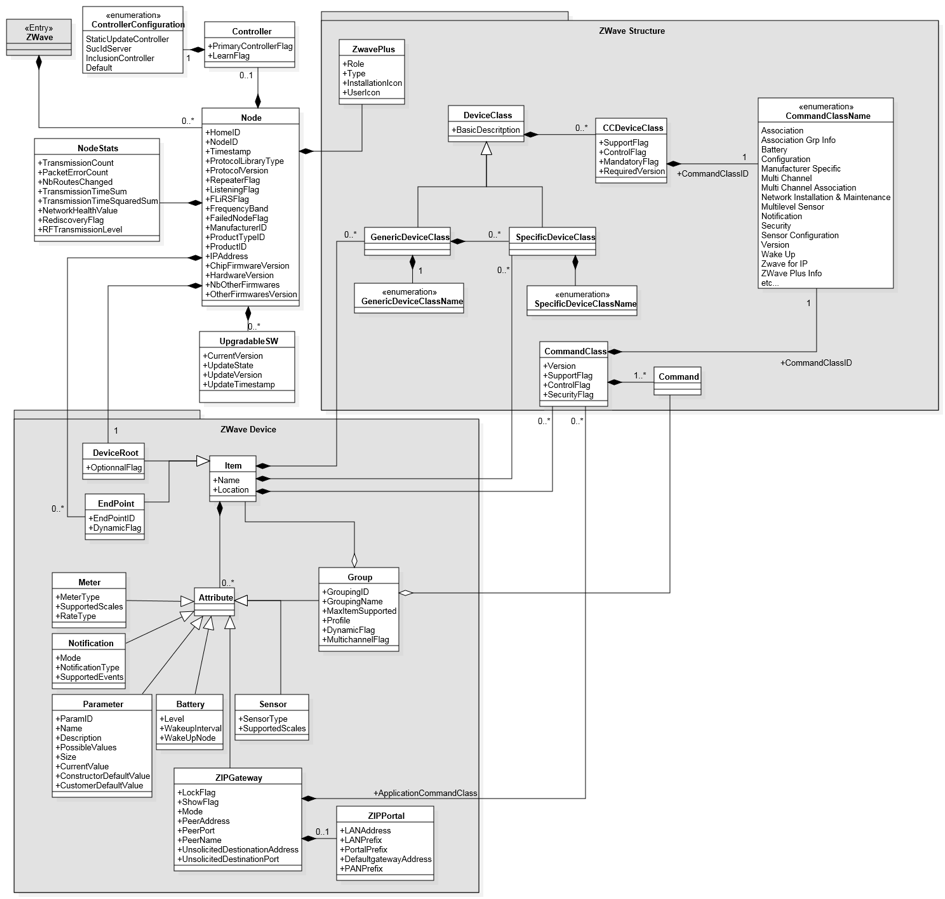
\includegraphics[width=14.5cm]{Figures/datamodel.png}
	\caption[Z-Wave Node Data Model]{Z-Wave Node Data Model}
	\label{fig:zwavedatamodel}
\end{figure}
%----------------------------------------------------------------------------------------
\section{Update Z-Wave in TR-069}
In order to retrieve the Z-Wave data from the Homelive Box, a http request to Homelive firmware can return a file (JSON or XML) which contains all the parameters that generated from lower layer. Then we should write a program to parser the file and save it in the TR-069 Client database.

\subsection{HTTP Request}
In addition to sending requests using standard UPnP, we can also do most things using a simple HTTP requests. Use the built-in URL data_request, and pass the following on the URL: \url{http://ip_address:3480/data_request?id=user_data&output_format=xml}.

This returns the configuration data for Vera, which is a list of all devices and the UPnP variables which are persisted between resets as well as rooms, names, and other data the user sets as part of the configuration.

In our case, we should retrieve the data of \textit{status}, so we change \textit{user_data} to \textit{status}. The http request is being called in the Homelive, so we can replace it with the local address: \url{http://127.0.0.1/}. And in consideration of parser, we set the output format to \textit{JSON}. The request url become:\\
\url{http://127.0.0.1:3480/data_request?id=status&output_format=json}

We can call this http request by using the API already provided in TR-069 Client:
\begin{lstlisting}[mathescape]
    int DM_HttpGetFile(IN httpGetFileDataType * httpGetFileDataPtr)
\end{lstlisting}

After this, we will have the JSON file in format of Luup data model, the next step is to parse the file.

\subsection{JSON Parser}
JSON parser is not a default library of language C, so we have to find a JSON parser. Fortunately, in the Luup firmware, there is a JSON parser library already included, which is \textit{json-c}. My program is based on \textit{json-c} library and use a iterative structure to parse the JSON file we retrieved from Luup( See Appendices 2).

After parse the JSON file, we will have a huge name\textbackslash value pairs, a two-dimension table is declared to saved them in buffer with dynamic memory management.

The next step is to find the correspondence between Z-Wave data model and Luup data model.

\subsection{Simple file Storage System}
TR-069 Client use simple file storage system as its data base. The structure is as following:

\begin{figure}[htbp]
	\centering
		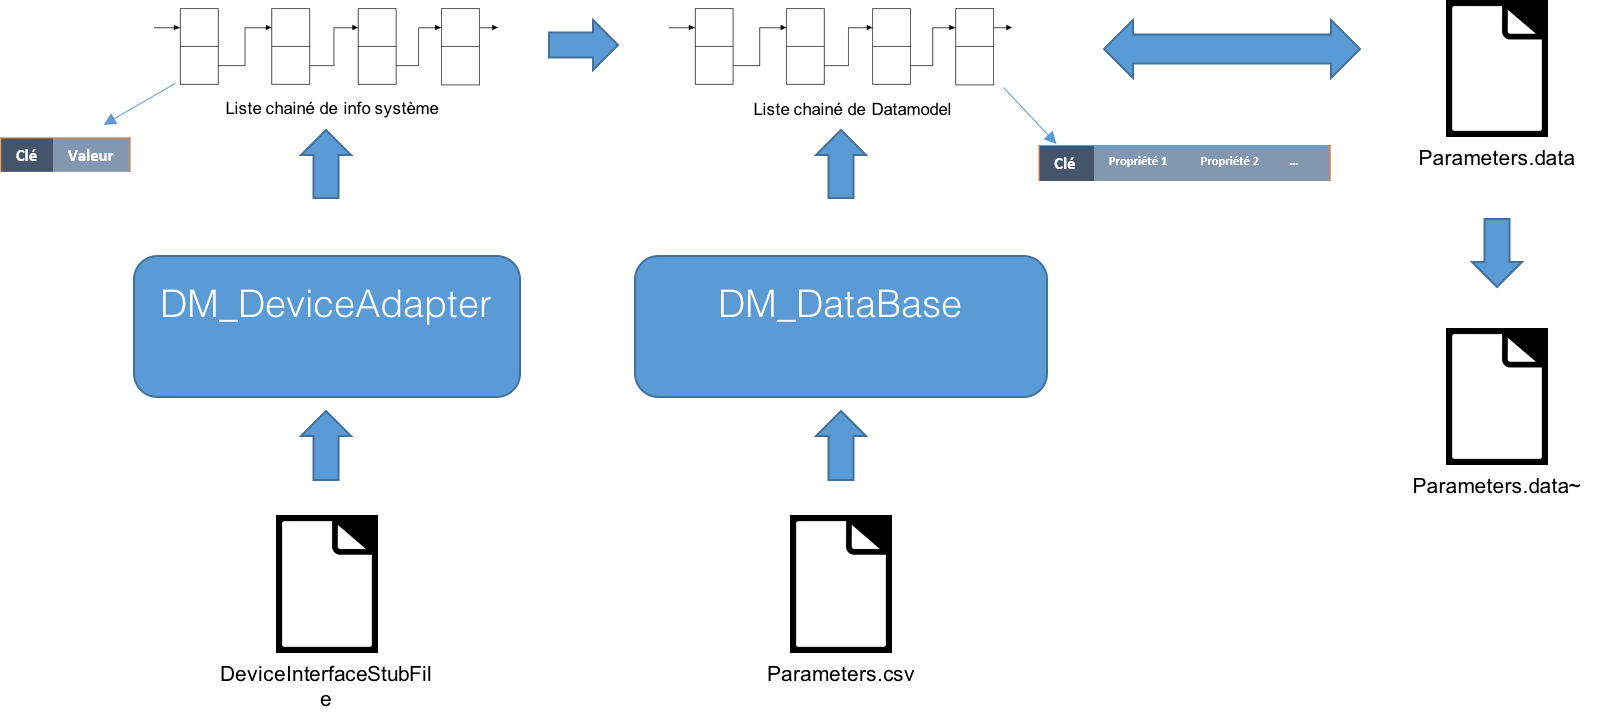
\includegraphics[width=14.5cm]{Figures/database}
	\caption[TR-069 Simple File Storage System]{TR-069 Simple File Storage System}
	\label{fig:database}
\end{figure}

When the program starts, there are two modules are in charge of manage the database. First is the module \textit{DM\_ DeviceAdapter}, it reads the configuration file \textit{DeviceInterfaceStubFile}, which contains the system parameters(Manufacturer, ProductClass, SerialNumber, etc..), and it will create a linked list to store the name\textbackslash value pairs.

After that, module \textit{DM\_ Database} will read the data model file \textit{parameters.csv} and build a linked list from it. In the \textit{parameters.csv}, there are name\textbackslash value of the data model and also 10 properties (Datatype, Writable, Notification type, etc..). When finish building the long linked list, it will read the value from the short linked list(\textit{DeviceInterfaceStubFile}) and copy them into the long linked list.

In the runtime, a file called \textit{parameters.data} will be created, and TR-069 will store all the data model in this runtime file in format of CSV (Comma-separated values) as the storage base.

The backup file is called \textit{parameters.data\~{}}, before every modification made to data model, the \textit{parameters.data} will save all the information into \textit{parameters.data\~{}} as a backup and update its own value.


\subsection{Synchronization Data model Luup and Z-Wave}

The data model of Luup and Z-Wave have different in approach but equally contains the data we need. For each data in Z-wave data model, we should find the correspondence in Luup data model. For example, in Luup there is a data called \textit{ZWave.devices.\{i\}.states.15.variable WakeupInterval}, the correspondence we found in Z-Wave is \textit{Device.Zwave.Interface.\{i\}.WakeUpInterval}. To synchronize the two data model, the value of \textit{WakeInterval} in Luup should be given to Z-Wave \textit{WakeInterval}. We have studied 100 parameters in Z-wave, and there are 27 are directly accessible from Luup data model, 26 can be calculated from Luup data model. For instance, the translation is finished for those all.

% Chapter 7

\chapter{Conclusion} % Main chapter title

\label{Chapter7} % For referencing the chapter elsewhere, use \ref{Chapter6}

\lhead{Chapter 7. \emph{Conclusion}} % This is for the header on each page - perhaps a shortened title

%----------------------------------------------------------------------------------------

The past six months of my internship have been very instructive for me. It's the first time that I participated in an industrial research project. This opportunity allows me to learn and develop myself in many areas. I gained a lot of experience, especially in CWMP and Z-Wave Protocol. A lot of activities are familiar with what I have learned at school. They enhanced my competence in computer science and inspired my interests in industrial research work.

On the other hand, I also encountered problems that I had never come across before. It was good to find out what my weaknesses are. This helped me to define which skills and knowledges I have to improve in the coming study time.

One thing I appreciate a lot is the DM2E meeting organized by group members. They invite researchers specialized in one particular area to share their opinions and ideas with other people. Even if I didn't understand all discussions, I did get a global picture for my unknown topics from these presentations. Such experience makes me eager to learn more and explore more; it really broadened my horizons.

From this internship I also learned the importance of time management. Once I realized what I had to do, I organized my day and work so that I did not waste my hours. A Gantt diagram of my internship helps with the time management.

This six-month internship passed too quickly. I am grateful for meeting so many wonderful staff members. I will try my best to apply all I learned here into my future careers and sincerely give all my best regards to my group members.


%----------------------------------------------------------------------------------------
%	THESIS CONTENT - APPENDICES
%----------------------------------------------------------------------------------------

\addtocontents{toc}{\vspace{1em}} % Add a gap in the Contents, for aesthetics

\appendix % Cue to tell LaTeX that the following 'chapters' are Appendices

% Include the appendices of the thesis as separate files from the Appendices folder
% Uncomment the lines as you write the Appendices

% Appendix A

\chapter{Installation of OptiX} % Main appendix title

\label{AppendixA} % For referencing this appendix elsewhere, use \ref{AppendixA}

\lhead{Appendix A. \emph{Installation of OptiX}} % This is for the header on each page - perhaps a shortened title

\lstdefinestyle{DOS}
{
    backgroundcolor=\color{black},
    basicstyle=\scriptsize\color{white}\ttfamily
    numbers=none,
    numbersep=8pt,                   % how far the line-numbers are from the code
    numberstyle=\tiny\color{white}, % the style that is used for the line-numbers
    stepnumber=1                    % the step between two line-numbers. If it's 1, each line will be numbered
}
%----------------------------------------------------------------------------------------
\lstdefinestyle{C}
{
  morekeywords={export}
}
%----------------------------------------------------------------------------------------

This appendix will introduce how to install and verify the correct operation of the OptiX Ray Tracing Engine. Since OptiX is a CUDA-based framework, this installation is composed of 2 steps: Installation of CUDA Toolkit and installation of OptiX SDK. Note that OptiX is not listed in the \textit{Logithèque} of \textit{Calibre 7} (a Debian based distribution developed at EDF); a root account during installation is required.

%----------------------------------------------------------------------------------------

\section{Pre-installation Actions}
Some verifications must be taken before the entire process of installation:

%----------------------------------------------------------------------------------------

\subsection{Verify the System Has a CUDA-Capable GPU}
First of all, as a GPU framework developed by Nvidia, OptiX requires a CUDA-supported device. To verify if your GPU is CUDA-capable, open your \textit{Terminal} and enter:
\begin{lstlisting}[style=DOS][language=bash]
  $ lspci | grep -i nvidia
\end{lstlisting}
If the shown GPU can be found in the following list: \href{http://developer.nvidia.com/cuda-gpus}{http://developer.nvidia.com/cuda-gpus}, it's CUDA-capable. Otherwise, you should look for another GPU.

%----------------------------------------------------------------------------------------

\subsection{Verify GCC Compiler}
The gcc compiler is generally installed as part of the Linux distribution. Either it was installed or should be installed manually by yourself, make sure the installed gcc is the same version which was used to build your Linux kernel (\fref{fig:gcc}), or you will surely get errors during next step. Confirm your Linux kernel information:
\begin{lstlisting}[style=DOS][language=bash]
  $ cat /proc/version
\end{lstlisting}
Using the following command in order to verify the version of gcc installed on your system:
\begin{lstlisting}[style=DOS][language=bash]
  $ gcc -v
\end{lstlisting}

\begin{figure}[htbp]
	\centering
		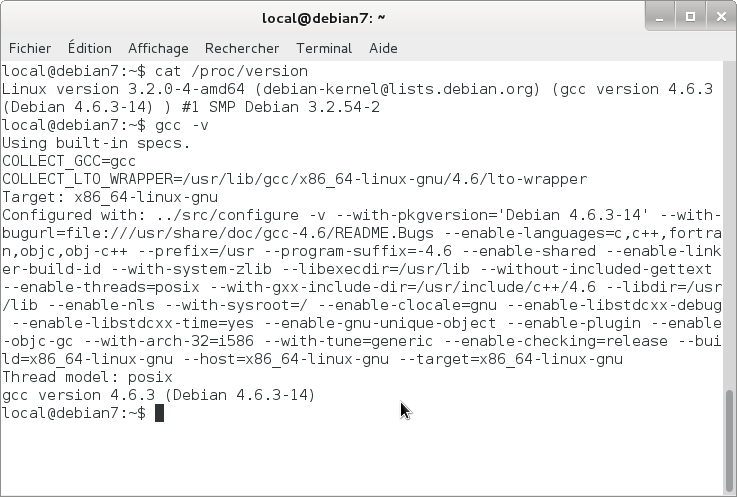
\includegraphics[width=13cm]{Figures/gcc.png}
	\caption{Verify the gcc compiler}
	\label{fig:gcc}
\end{figure}
After all these actions done, the installation can be continued to the next step.

%----------------------------------------------------------------------------------------

\section{Installation of CUDA Toolkit}
The NVIDIA CUDA Toolkit is available at \href{https://developer.nvidia.com/cuda-toolkit-archive}{https://developer.nvidia.com/cuda-toolkit-archive}. Choose and download the distribution-independent package ("RUN" package) for Ubuntu distribution, which corresponds to the \textit{Calibre} system. Notice that any architecture of CUDA is running based on a supported driver, for which an update is highly recommended. Although a driver update module is integrated in the CUDA installation package, it turns out not to be convenient for users: updates crash without any warning information. Therefore, one practical choice is to install respectively these two parts. Here we take a Nvidia Quadro FX 1800 as an example and install CUDA 5.5.22.
%----------------------------------------------------------------------------------------

\subsection{Installation of the NVIDIA Driver}
With the GPU information checked before, download the latest driver installation package: \href{http://www.nvidia.com/Download/index.aspx?}{http://www.nvidia.com/Download/index.aspx?}. In order to update a GPU driver, one should drop graphics interface on pressing \textit{Ctrl+Alt+F1} and stop \textit{X} server:
\begin{lstlisting}[style=DOS][language=bash]
  $ service gdm3 stop
\end{lstlisting}
To make the package executable, run the following:
\begin{lstlisting}[style=DOS][language=bash]
  $ sudo chmod x NVIDIA-Linux-x86_64-331.49.run
\end{lstlisting}
Install the NVIDIA driver on performing:
\begin{lstlisting}[style=DOS][language=bash]
  $ sudo ./NVIDIA-Linux-x86_64-331.49.run
  $ sudo reboot
\end{lstlisting}
Verify the driver has been successfully installed:
\begin{lstlisting}[style=DOS][language=bash]
  $ cat /proc/driver/nvidia/version
\end{lstlisting}

%----------------------------------------------------------------------------------------

\subsection{Installation of CUDA Toolkit}
Quit GUI on pressing \textit{Ctrl-Alt-F1} and begin installation by executing:
\begin{lstlisting}[style=DOS][language=bash]
  $ cat service gdm3 stop
  $ sudo chmod a+x cuda_5.5.22_linux_64.run
  $ sudo ./cuda_5.5.22_linux_64.run
\end{lstlisting}
Then the environment variables for our operating system need to be changed on editing the \textit{.bashrc} file:
\begin{lstlisting}[style=DOS][language=bash]
  $ gedit .bashrc
\end{lstlisting}
Add these two lines on the top of the current file and save:
\begin{lstlisting}[style=C]
    export PATH=/usr/local/cuda-5.5/bin:$PATH
    export LD_LIBRARY_PATH=/usr/local/cuda-5.5/lib64:$LD_LIBRARY_PATH
\end{lstlisting}


%----------------------------------------------------------------------------------------

\subsection{Verify the Installation of CUDA}
Before continuing, it is important to verify that the CUDA Toolkit can find and communicate correctly with the CUDA-capable hardware. To do this, you need to compile and run some sample programs.
Changing to the sample directory and compiling the examples:
\begin{lstlisting}[style=DOS][language=bash]
  $ cd ~/NVIDIA_CUDA-5.5_Samples 
  $ make
\end{lstlisting}
After compilation, run \textit{deviceQuery} and observe the result:
\begin{lstlisting}[style=DOS][language=bash]
  $ cd ~/NVIDIA_CUDA-5.5_Samples/bin/linux/release 
  $ ./deviceQuery
\end{lstlisting}
The output of this executable should look similar to the \fref{fig:cudatest}. Note that the important outcomes are that a device was found (the first highlighted line), that the device matches the one on your system, and that the test passed successfully (the second highlighted line).
\begin{figure}[htbp]
	\centering
		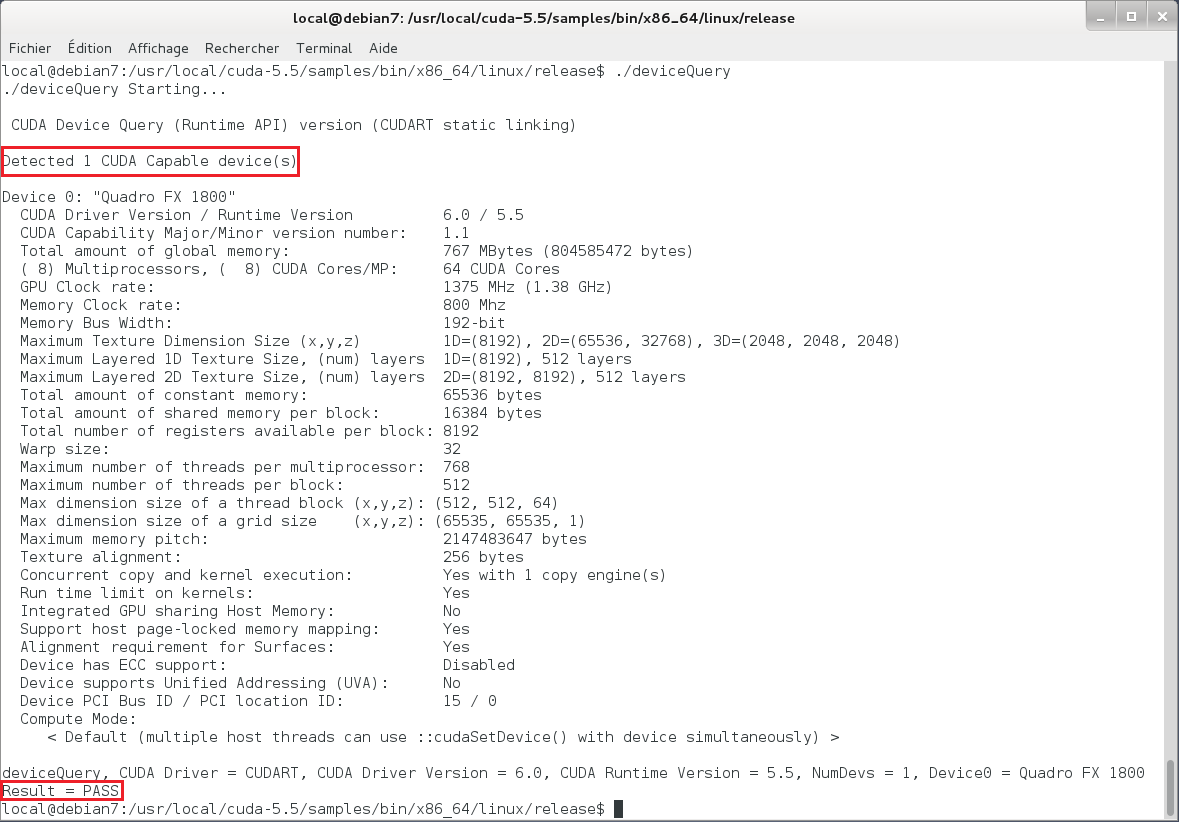
\includegraphics[width=13cm]{Figures/cudatest.png}
	\caption{CUDA test result}
	\label{fig:cudatest}
\end{figure}
%----------------------------------------------------------------------------------------

\section{Installation of OptiX SDK}
Unlike CUDA, there is no direct link to download an OptiX installation package. All developers need to create a special account: \href{https://www.surveymonkey.com/s/3D9FLR6}{https://www.surveymonkey.com/s/3D9FLR6}, two or three days later you will receive an email with your username and password inside. Then go to: \href{https://ftpservices.nvidia.com}{https://ftpservices.nvidia.com} and download corresponding installation package. Since the registration may take long, you can get a direct access with following coordinates:
\begin{itemize}
  \bf
  \item Username: OptiX-Beta-137
  \item Password: OptiX-Prime-Raytracing
\end{itemize}
To fully explore all features of OptiX, we choose to install the latest release at present: OptiX 3.5.1. Run the installation package:
\begin{lstlisting}[style=DOS][language=bash]
  $ sudo chmod a+x NVIDIA-OptiX-SDK-3.5.1-linux64.run
  $ sudo ./NVIDIA-OptiX-SDK-3.5.1-linux64.run
\end{lstlisting}
%----------------------------------------------------------------------------------------

\subsection{Post-installation Setup}
Establish links to OptiX library files:
\begin{lstlisting}[style=DOS][language=bash]
  $ sudo ln -s /home/local/NVIDIA-OptiX-SDK-3.5.1-PRO-linux64/lib64/liboptix.so.1 /usr/lib/liboptix.so.1
\end{lstlisting}
\begin{lstlisting}[style=DOS][language=bash]
  $ sudo ln -s /home/local/NVIDIA-OptiX-SDK-3.5.1-PRO-linux64/lib64/liboptixu.so.1 /usr/lib/liboptixu.so.1 
\end{lstlisting}
\begin{lstlisting}[style=DOS][language=bash]
  $ sudo ln -s /home/local/NVIDIA-OptiX-SDK-3.5.1-PRO-linux64/lib64/liboptix_prime.so.1 /usr/lib/liboptix_prime.so.1 
\end{lstlisting}

%----------------------------------------------------------------------------------------

\addtocontents{toc}{\vspace{1em}} % Add a gap in the Contents, for aesthetics
% Appendix B

\chapter{JSON parser in C} % Main appendix title

\label{AppendixB} % For referencing this appendix elsewhere, use \ref{AppendixA}

\lhead{Appendix B. \emph{JSON Parser in C}} % This is for the header on each page - perhaps a shortened title
%--------------------------------------------------------------------

\addtocontents{toc}{\vspace{1em}} % Add a gap in the Contents, for aesthetics
%% Appendix C

\chapter{Time Management} % Main appendix title

\label{AppendixC} % For referencing this appendix elsewhere, use \ref{AppendixA}

\lhead{Appendix C. \emph{Time Management}} % This is for the header on each page - perhaps a shortened title

\lstdefinestyle{DOS}
{
    backgroundcolor=\color{black},
    basicstyle=\scriptsize\color{white}\ttfamily
    numbers=none,
    numbersep=8pt,                   % how far the line-numbers are from the code
    numberstyle=\tiny\color{white}, % the style that is used for the line-numbers
    stepnumber=1                    % the step between two line-numbers. If it's 1, each line will be numbered
}
%----------------------------------------------------------------------------------------
\lstdefinestyle{C}
{
  morekeywords={export}
}
%----------------------------------------------------------------------------------------

This appendix presents a task list through the practice period and its corresponding Gantt diagram.

Generally speaking, most tasks were finished as they had had been scheduled. Especially in the first two months, time spent on bibliography work was much less than it had been estimated. 

Major delay came from the implementation of object-oriented programming on GPUs and dynamic allocations. This part of work should have been done within one month. Unfortunately, it hasn't been finished during the internship. To a certain extent, other reasons like no available working computer in the first week or contacting researchers in the USA for technical supports postponed the advancement as well. Furthermore, the report redaction lasted for about one month.
\begin{figure}[htbp]
	\centering
		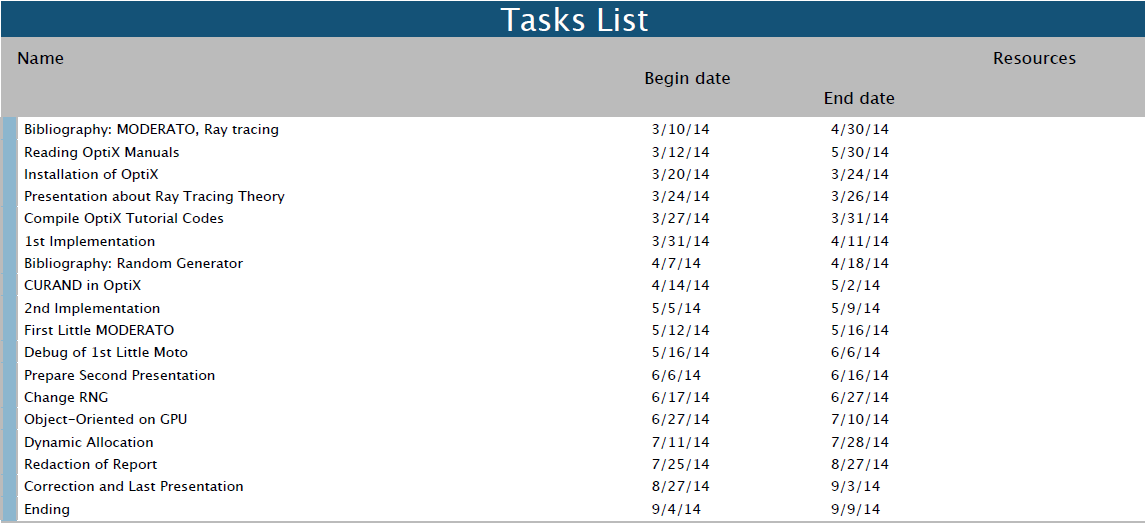
\includegraphics[width=10cm]{Figures/task.png}
	\caption{Task list.}
\end{figure}
\begin{figure}[htbp]
	\centering
		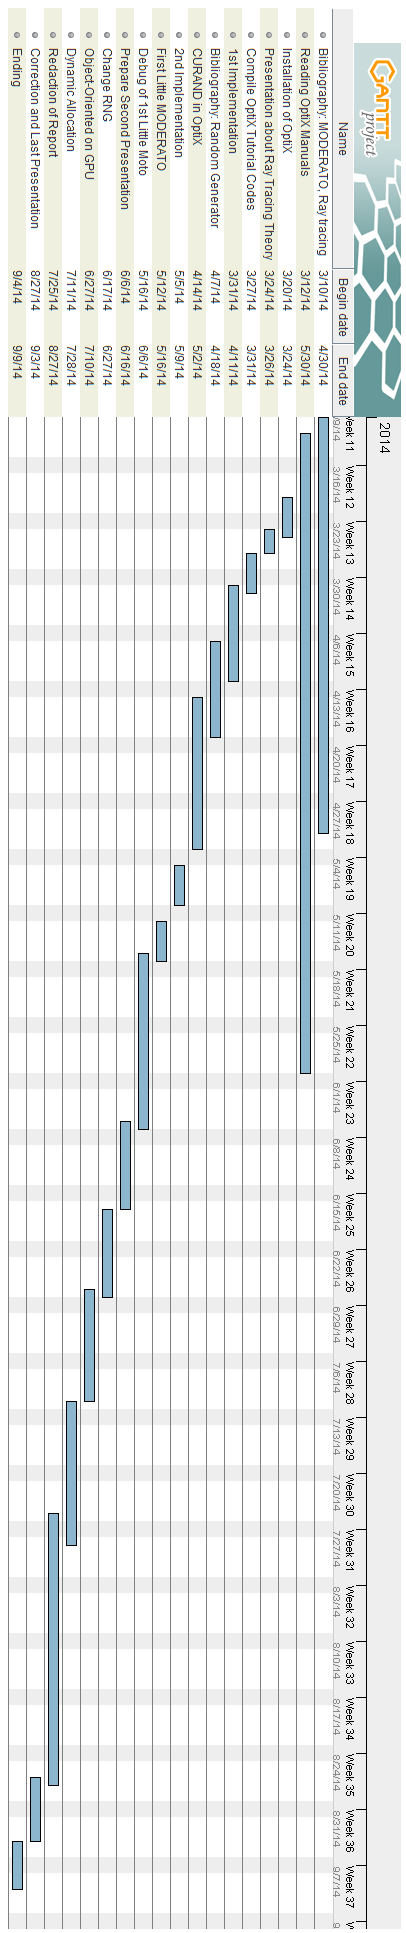
\includegraphics[width=\textwidth,height=\textheight,keepaspectratio]{Figures/report.png}
	\caption{Gantt diagram.}
\end{figure}

%\addtocontents{toc}{\vspace{1em}} % Add a gap in the Contents, for aesthetics

\backmatter

%----------------------------------------------------------------------------------------
%	BIBLIOGRAPHY
%----------------------------------------------------------------------------------------

\label{Bibliography}

\lhead{\emph{Bibliography}} % Change the page header to say "Bibliography"

\bibliographystyle{unsrtnat} % Use the "unsrtnat" BibTeX style for formatting the Bibliography

\bibliography{Bibliography} % The references (bibliography) information are stored in the file named "Bibliography.bib"

\addtocontents{toc}{\vspace{1em}} % Add a gap in the Contents, for aesthetics

%----------------------------------------------------------------------------------------
%	ABSTRACT PAGE
%----------------------------------------------------------------------------------------
\setstretch{1.5} % Reset the line-spacing to 1.5 for body text (if it has changed)

\clearpage % Start a new page

\frontmatter % Use roman page numbering style (i, ii, iii, iv...) for the pre-content pages

\abs{\addtocontents{toc}{\vspace{1em}} % Add a gap in the Contents, for aesthetics

The TR-069 developed by Orange Labs allows to manage communication between customer-premises equipment (CPE) and Auto Configuration Server (ACS).It offers the use of a set of services administration, monitoring and diagnosis while avoiding the problems associated with hardware and software diversity.

Orange Homelive is the solution to manage the home on the mobile. From a single application, Homelive allows to interact with connected compatiable objects in the house. It proposes the Smart Home solution with a set-top box--Homelive.

Z-Wave is a wireless protocol designed for home automation (lighting, private heating) and so-called Smart Home. Z-Wave was bought by the company Americane Sigma Designs in 2008. It is optimized for low bandwidth exchanges and devices on battery. It can be easily integrated in consumer electronics, including remote controls, smoke detectors and safety sensors.

During the six-month internship, my main mission was to adapt the TR-069 Client at the Homelive box by resolving the incompatibility and implementing the RPC methods. Also, integrates the new Z-Wave data model in the TR-069 Client by contacting with the Luup firmware of the Homelive Box. With my internship result, Orange will be allowed to manage Homelive from distance to reduce the expenses on support services.
}

%----------------------------------------------------------------------------------------
%	RÉSUMÉ PAGE
%----------------------------------------------------------------------------------------

\clearpage % Start a new page

\resume{\addtocontents{toc}{\vspace{1em}} % Add a gap in the Contents, for aesthetics

Le TR-069 développé par Orange Labs permet de gérer la communication entre un équipement terminal du réseau local du client et un servert d'autoconfiguration associé dans un même réseau apprtenant à l'opérateur.Il offre à l'utilisation d'un ensemble de services d'administration, de contrôle et de diagnostic tout en évitant les problèmes liés aux diversités matérielles et logicielles.

Orange Homelive est la solution pour piloter sa maison depuis son mobile. A partir d'une seule application, Homelive permet d'interagir avec les objets connectés compatiables dans la maison. Il donne la solution de Smart Home avec un set-top box--Homelive.

Z-Wave est un protocole radio conçu pour la domotique(éclairage, chauffrage) et ce qu'on appelle l'Habitat comminicant. En 2008 Z-Wave a été rachetée par la société américane Sigma Designs. Il est optimisé pour des échanges à faible bande passante et des appareils sur pile ou alimentés électroniquement. Il peut être facilement intégrée dans les produits électroniques de consommation, y compris télécommandes, les détecteurs de fumée et capteurs de sécurité.

Pendant ces six mois de stage, ma mission principale a été d'adapter le TR-069 Client au Homelive box, en résoulvant les incompatibilité et implémentant les RPC méthodes. Ainsi que intégre le nouveau data modèle Z-Wave dans le TR-069 Client en communiquant avec le firmware Luup dans Homelive Box. Avec mon résultat de stage, Orange va être autorisé à gérer Homelive à distance pour réduire les dépenses sur les services de soutien.
}

%----------------------------------------------------------------------------------------
\end{document}
